\documentclass[]{final_report}

\def\studentname{Stephen Lennon}
\def\projecttitle{Application Replay for Performance Evaluation and Tuning}
\def\supervisorname{Dr. Liam Murphy}

\begin{document}

\maketitle

%% Abstract %%
\begin{abstract}

When a program is executed in the Java Virtual Machine it is ordinary that factors including thread scheduling, the capacity of the executing machine, pseudorandom number sources and inputs to the program cause it to execute differently each time it is run. While ordinarily desirable that a program should react to external factors there is utility in making the program repeat a specific execution path for the purposes of functional testing. This project builds upon existing techniques of \textit{Bytecode Replay} to construct a new technique here coined \textit{Application Replay} which applies modern Java techniques of runtime instrumentation and bytecode engineering to record and replay input to a Java application by instrumenting selected methods while leaving the operation of the application otherwise free to adapt to external factors.

This technique is then used to create a framework capable of invoking the application repeatedly for the purposes of performance measurement. It is proposed that the application which is disconnected from its normal source of input can be run repeatedly to test the performance implications of different combinations of parameters passed to the Java Virtual Machine, and that this can be done programmatically and in isolation from other systems on which the application is normally dependant once it is placed in Application Replay mode.

\end{abstract}
\newpage

\clearpage
\pdfbookmark{Table of Contents}{toc}\tableofcontents
\newpage

\clearpage
\pdfbookmark{Figures}{figures}\listoffigures
\newpage

\clearpage
\pdfbookmark{Listings}{listings}\lstlistoflistings
\newpage

%% Introduction %%

\chapter{Introduction \label{introduction}}

Since before the advent of Cloud Computing or the Java programming language, the difficulty of reasoning about the execution of distributed systems has been studied. The challenges of debugging distributed computer programs compared to sequential deterministic programs was sumarised by Leblanc and Mellor-Crummey (1987)\cite{leblanc:1987} who said ``Debugging parallel programs is considerably more difficult because successive executions of the same program often do not produce the same results\ldots{}Methods to reproduce the execution typically require that the contents of each message be recorded in an event log as it is received.'' The \textit{results} referred to here are specifically errors manifested in the execution of the program, that may not occur on every execution, however the solution proposed: to record, and later replay messages within the application for the purpose of reproducing the execution of the program has potentially many applications.

Since the inception of Amazon Web Services\footnote{\url{http://aws.amazon.com}} in 2002 and its later evolution into a general purpose consumer cloud computing platform in 2006,\cite{pallis:2010} cloud computing in its current form has proliferated, and with it, the fate of sequential deterministic applications is sealed. Papazoglu \cite{papazoglou:2008} cites \textit{elasticity} as an ``Essential characteristic of Cloud Computing" in that more computers, referred to as \textit{instances}, can be added automatically to meet the load and performance requirements of a distributed cloud application. It seems evident that, if this elasticity is exploited to its full potential then a problem of a poorly performing system could be masked by having too many instances running the distributed application, however running a performance test against the application means that all upstream applications from which it draws inputs also experience elevated load, possibly interfering with the availability of the system for production use, and the state of the system may be undesirably changed. For this reason performance tests are usually conducted on a separate dedicated performance testing environment that forms a complete copy of all components required by an application under test. Because such performance testing environments are expensive to maintain, scheduling availability for testing can be a challenge. One statistic from 2011,\cite{jenkins:2011} states that software changes to Amazon's production systems that run their retail services around the world happen at an average of one deployment every 11.6 seconds on weekdays over the month of May 2011. That represents a very large number of changes to a large heterogeneous application, and it is hard to envision a traditional approach to performance testing being effective.

On the other hand, if the system undergoing change were decoupled from its dependencies such that it could be run in isolation then placing it under load could affect no other system, either by placing that other system under load or by introducing test data into other systems, and it would seem that an implementation of message record and replay should be explored as a means to effect that decoupling.

\begin{figure}
\begin{center}
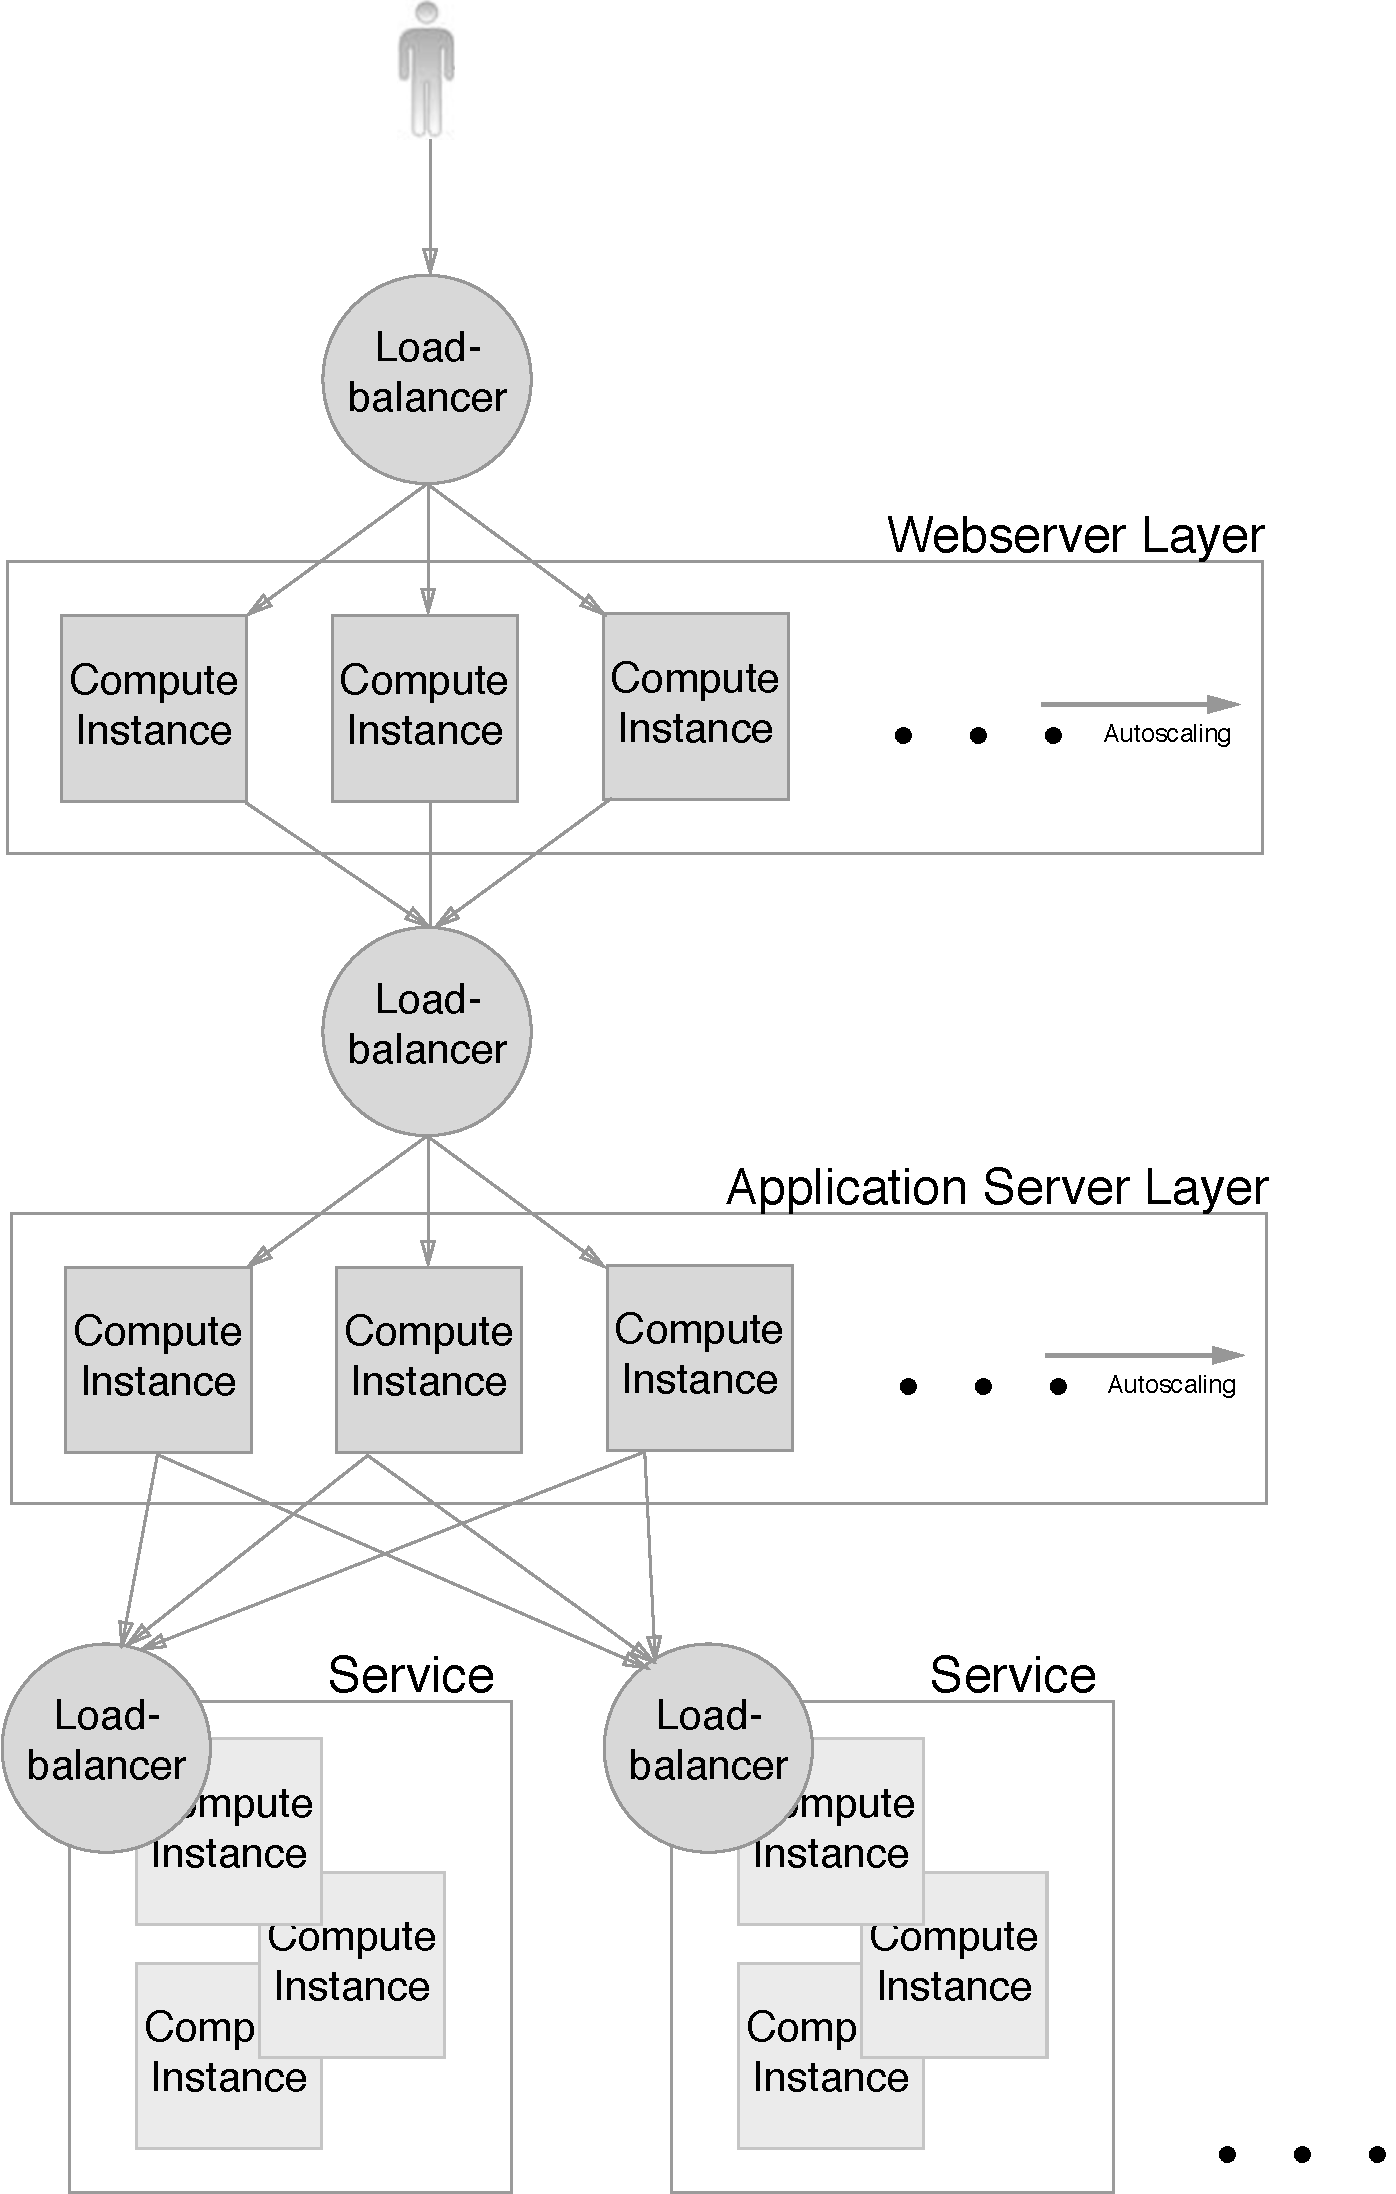
\includegraphics[scale=0.3]{figures/Webservice_fig.pdf}
\caption{\small \sl Simplified Typical Web Services Architecture \label{fig:webservice_architecture}}
\end{center} 
\end{figure}

Figure \ref{fig:webservice_architecture} shows a typical large application designed for horizontal (possibly automatic) scaling, whereby layers of the application can be scaled by the addition of more instances.\cite{el:2005} The \textit{Application Server Layer} is in turn dependant on other web services accessible to it, and those dependencies may, in turn, have a similar architecture or may be constructed in an entirely different fashion. This project includes a sample Representational State Transfer (REST) web service that fits into the \textit{Application Service Layer} of the scheme depicted, having a dependency on an external service. The process of decoupling the provided sample application from its dependency and performing experiments to evaluate its performance is addressed in the remainder of this paper.

As this project deals with the Java language, we can consider that capturing the essential information contained in a method call addresses the requirement to capture messages as explained by Leblanc and Mellor-Crummey (1987)\cite{leblanc:1987} and so rapidly the task of application replay in Java appears to overlap significantly with existing techniques of bytecode replay where it is defined to include input replay such as in the \textit{jRapture} \cite{steven:2000} and \textit{Scarpe} \cite{joshi:2007} tools discussed in Chapter \ref{related_work}.

The objective of this project is to examine potential ways to automate performance tuning. Specifically focusing on the exploration of Java Virtual Machine parameters in an effort to locate combinations of parameters that provide preferable performance characteristics when running an application that has been decoupled from its dependencies. To this end an examination of the available JVM parameters was conducted, and a subset of parameters determined to form the basis of experimentation. A range of values was chosen for each such parameter: \textit{true} or \textit{false} for boolean parameters; an incrementing range of integers or a list of strings. As part of this project, the Garbage Collector related parameters were scrutinised to limit the number of sensible combinations, thereby making automated testing more efficient. All remaining selected parameters are combined in all combinations and a target process is executed using each such combination.

In each experimental run of the target application, key performance metrics are extracted from the target JVM using the Java Management Extensions (JMX) server built in to the Oracle HotSpot JVM. For the duration of the application run, these key performance metrics are collected in time series and they are then used to assign a simple performance score and to produce graphs of the test execution.

\section*{Project Artefacts}

\begin{figure}
\begin{center}
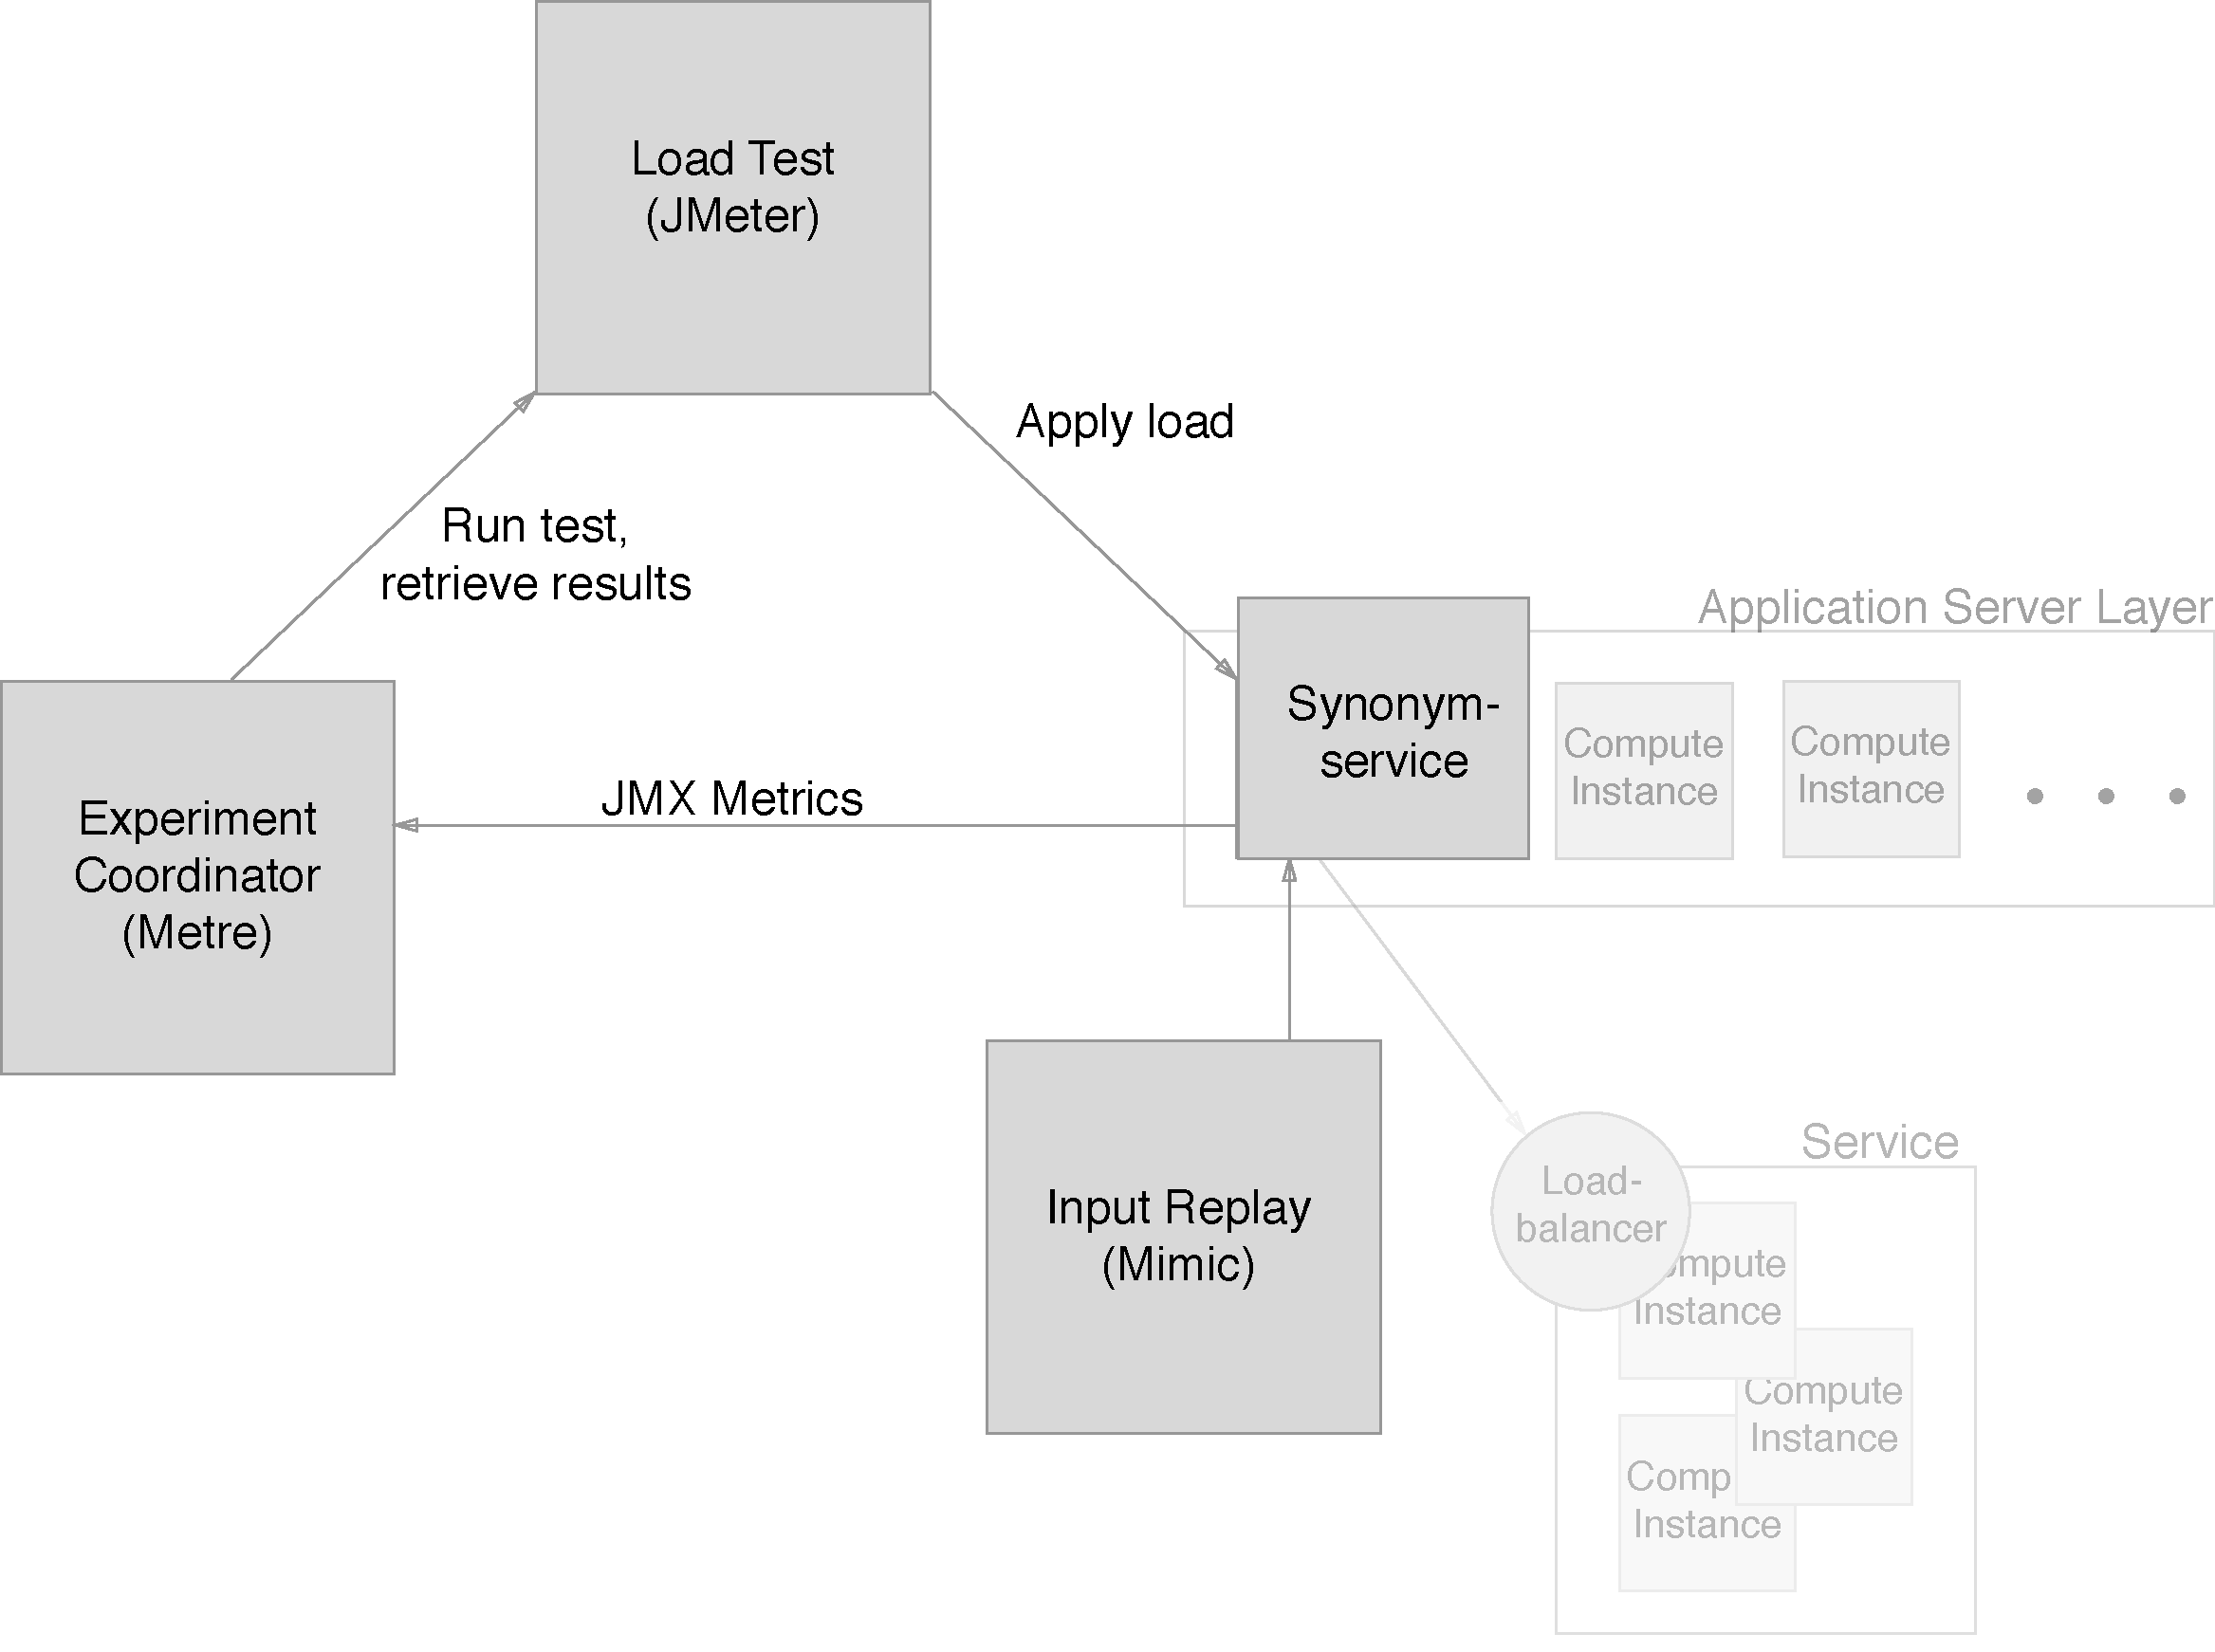
\includegraphics[scale=0.3]{figures/Scheme_fig.pdf}
\caption{\small \sl Interaction of Project Artefacts \label{fig:scheme}}
\end{center}
\end{figure}

In order to conduct the performance experiments described, a total of three major project artefacts are produced as shown in Figure \ref{fig:scheme}, these are now briefly outlined.

\subsection*{The \textit{Synonym Service} Sample Application}
The Synonym Service is built using the Spring Boot application framework\footnote{\url{http://projects.spring.io/spring-boot/}} to provide a small but complete REST web service that accepts a block of text and attempts to construct another block of text with the same message digest, where BSD Sum and MD5 digests are selectable. Both the original text and the resulting text then have the same message digest, but the text is different\cite{daum:2005}. The technique employed is to replace words in the original text with different words that have similar meaning. These synonyms are drawn from an external upstream service provided by the company \textit{Big Huge Labs}\footnote{\url{https://words.bighugelabs.com}}. The Mimic artefact can then be used to provide an application replay mechanism that allows the Synonym Service to operate disconnected from this upstream service such that a JMeter test script can be run upon the service without generating any upstream calls.

\subsection*{The \textit{Mimic} Record and Replay Agent}
The Mimic agent is a Java agent that can be loaded into the JVM at startup using the \lstinline{-javaagent}\noop{} command line parameter to the Oracle Hotspot JVM\cite{java:2016}. Whichever application is loaded by the JVM, as specified on the command line also, will be instrumented by the Mimic agent. Mimic instruments classes and methods therein, as specified in its configuration file, to record invocations of the nominated methods (if invoked with the \textit{record} parameter), or to replay a previously recorded schedule (if invoked with the \textit{replay} parameter). It also applies instrumentation to the \lstinline{java.lang.Thread}\noop{} class to record a thread schedule that serves to identify threads on replay. This step is required because the JVM makes no attempt to keep the identifiers of threads identical across multiple runs of the application.

Where the configuration file of the Mimic agent specifies a class and method name that matches a method loaded into the JVM, that method is allowed to run unperturbed during the record phase to produce a schedule of output, and all functionality of the method is preserved so as to obtain a correct return value. The parameters to the method, the return value, and the running duration of the method are recorded in addition to some identifying static information. Upon replay the method is \textit{short-circuited}, in that the original functionality within the method is replaced with a stub that replays the originally recorded return value. The running duration of the method, when it ran originally, is simulated also with an artificial delay. Importantly though, any upstream call that the method performed no longer occurs, and so, given careful selection of methods in the Mimic configuration file, upstream dependencies can thus be disconnected to isolate the application component under test.

\subsection*{The \textit{Metre} Experiment Coordinator}
The Metre application is provided to conduct performance experiments on the application that has been disconnected using the Mimic agent. Because this project aims to find the most performant  set of JVM parameters from a defined search space, the configuration file of the Metre application defines the search space of JVM parameters to be explored. The Metre application then iterates through this search space, producing a list of JVM parameters on each iteration and invokes the application under test, which, in this case, is the instrumented Synonym Service.

Simulatneously Metre starts an instance of Apache JMeter\footnote{\url{http://jmeter.apache.org}} and runs the test script defined in its configuration file to load the target. Upon completion of the JMeter test run, the results of the test are extracted from the JMeter log file produced.

As the application runs and is subjected to load, Metre also connects to the Java Management Extensions server of the JVM in which the target application is running.

After all combinations of JVM parameters have been exercised, the individual results are sorted and the top \textit{n} results are selected as determined by a score based on the run time of the experiment, where \textit{n} is specified in the Metre configuration file. For each of the top \textit{n} runs, a Gnuplot\footnote{\url{http://www.gnuplot.info}} format file is produced on disk which contains a graph of the critical CPU and memory metrics throughout the performance experiment, and other key data such as Java Garbage Collector metrics.

%% Related Work %%
\chapter{Related Work \label{related_work}}
The idea of replaying the execution of an application has existed for some time, though the intent of the term \textit{replay} varies somewhat in related prior works. In the earliest work of sufficient relevance to include, LeBlanc and Mellor-Crummey (1987) \cite{leblanc:1987} define a technique of \textit{Instant Replay} in which they propose to replay all synchronisation activity in a program thereby making the execution of a highly parallel program deterministic and repeatable for the purpose of debugging. Interesting in this approach is the definition of \textit{messages} as events that carry information in a loosely coupled system, which can be recorded in an event log to effect replay. The authors then evolve this technique to tightly coupled systems and abandon the requirement to record the data passed in messages. Instead their technique is based on enforcing the ordering of synchronisation events, and so diverges from input replay.

Choi and Srinivasan (1998)\cite{choi:1998} present the DejaVu tool to make program execution deterministic by creating thread schedules of synchronisation events in the program, implemented as a modified Sun JVM. DejaVu uses a global and per-thread clock to record contiguous \textit{intervals} during which a thread is executing, bounded by synchronisation events, and reproduces it by replaying the synchronisation events.

Chiba (2000) \cite{chiba:2000} describes the \textit{Javassist} framework which provides structural reflection to complement behavioural reflection in Java. This allows changes to the structure of classes in the program at the time that they are loaded into the JVM. This is important to this work because Javassist is one of the frameworks evaluated to change the behaviour of methods to include record and replay functionality, as later described, and to effect small structural changes such as the addition of member variables required to support these modifications. This project instead employs the similarly capable \textit{ASM} framework for bytecode manipulation as described by Kuleshov (2007) \cite{kuleshov:2007}.

Steven et al. (2000) \cite{steven:2000} describe the \textit{jRapture} tool thus ``jRapture captures interactions between a Java program and the system, including GUI, file, and console inputs, among other types, and on replay it presents each thread with exactly the same input sequence it saw during capture.'' The purpose of this capture is to allow a human tester to record a sequence of execution through a program which can later be analysed statistically or by a developer of the program. An interesting point about jRapture is that it does not attempt to preserve threading schedules for replay because the intent of the application, to replay user-driven test sequences, is not dependant on thread scheduling, and there is no strong focus on the debugging of concurrency related issues. This overlaps with a premise of this project, in that the reproduction of thread scheduling is not required during replay for the purposes of performance measurement, in fact it is specifically undesirable.

Two other factors distinguish jRapture from the work here presented: jRapture is implemented by modifying the Java API and supporting libraries, whereas Mimic is implemented entirely without modification to the JVM or Java libraries, instead using load-time bytecode manipulation with ASM. Also, jRapture aims to define the points at which record and replay is conducted, specifically ``The implementation of jRapture includes modified versions of the Java API classes that interact directly with the underlying operating system or windowing system, such as FileInputStream, FileOutputStream, RandomAccessFile, Socket, DatagramSocket, and GUI component peer classes like MComponentPeer.'' \cite{steven:2000} Mimic, on the other hand, is designed for non-GUI, console applications and web services, and allows the user to select specific methods for record and replay. This places the onus on the user of Mimic to know which methods connect to other services and serve as input to the application under test but provides greater flexibility and potentially much less overhead in that, with proper configuration, Mimic only records the connection to upstream systems.

jRapture has a requirement to ensure that the same thread as produced a recorded event is the thread to receive it upon replay. The JVM provides no assistance in that the thread identifier can change when the application is replayed. jRapture identifies threads based on the following observation: ``Although threads may not be created in the same absolute order during capture and replay, each thread should create its children (threads) in the same order.'' \cite{steven:2000} Unfortunately, in the context of Mimic, threads may require recorded input before they have created their children. Mimic address the thread identification issue by generating a thread identifier independent of the JVM and based on the stack trace at the point that \lstinline{Thread.start()} is called. \noop{} This stack trace identifies the caller of each method, by class and line number recursively back through the execution stack.

Georges et al. (2002) \cite{georges:2002} describes the JaRec tool, which, like DejaVu (and unlike jRapture and Mimic) does not record input. Rather it assigns a distinct and incrementing number to each thread upon every synchronisation event to reproduce the order of thread execution in a multithread program. It is noteworthy though in that it is the first tool encountered that uses load-time bytecode instrumentation, a technique adopted for Mimic. Predating Java SE 5.0, it uses the Virtual Machine Profiling Interface (JMPI) instead of the more modern Virtual Machine Tool Interface, and so must run in a second JVM, separate from the application under test, and uses the Bytecode Engineering Library (BCEL)\footnote{\url{https://commons.apache.org/proper/commons-bcel/}} to effect manipulation of the bytecode.

As noted, jRapture integrates with the target application using a modified Java API, and the points of integration are a part of its design. The Scarpe tool described by Joshi and Orso (2007) \cite{joshi:2007} is noteworthy in that it allows the user to define a \textit{subsystem of interest}. It then automatically plots the boundary of that subsystem and effects record and replay functionality for interactions that cross the boundary. For the purposes of implementing Mimic, the ability to define a boundary is not of utility because the boundary of a web service is the boundary of the Java program, and it is not desired to record \textit{all} interactions across the boundary, only those with upstream systems. Thus Mimic configuration includes a user-specified collection of Java methods to serve as points of record and replay. Scarpe makes an effort to reduce the volume of data recorded by limiting focus to primitive values inside objects travelling over the boundary, an effort that is not required in the Mimic approach of defining interactions at a method level. Scarpe includes additional functionality that is not included in Mimic in that it can serve as a driver of the system under test, performing effectively the same function as the JMeter script used to apply load to the target application in this project.

Schuppan, Baur and Biere (2005)\cite{schuppan:2005} describe the format of a thread schedule that can achieve deterministic replay, but merely mention that the schedule could accommodate a record of the input to the program. The thread schedule is essential in Mimic as it serves to determine, during the replay phase, which thread receives the input that has been recorded.

This project aims to use bytecode manipulation at class-load time to effect input replay in a manner that most resembles that of jRapture. Matching of threads on record and replay is required to accommodate multi-threaded applications. The ASM bytecode manipulation framework is used at class-load time exploiting the Java Virtual Machine Tool interface. Recordings made with the Mimic tool are portable to other JVMs. To demonstrate the utility of the application replay facility of Mimic, the complementary Metre framework for performance experimentation is provided, and performance experiments are documented in Chapter \ref{results_and_analysis}.

Chapter \ref{system_description} provides a description of the Mimic application replay tool and documents some of the challenges of its development, and also the Metre performance experimentation tool that uses JMeter and Mimic to conduct performance experiments to tune JVM parameters.

Chapter \ref{experimental_design} describes the sample application \textit{Synonym Service} that serves as a the target of the performance expeiment, the configuration of the experiment and test environment.

Chapter \ref{results_and_analysis} and the remainder of the document describes the learnings and outcomes of the design and implementation of the project artefacts, including areas that were successful and those that did not perform as expected.


%% System Description %%
\chapter{System Description \label{system_description}}

%%%% Section for each artefact, focused on prior work, then my work %%
\section{Application Replay \label{application_replay}}

Both Steven et al. (2000) \cite{steven:2000} and Joshi and Orso (2007) \cite{joshi:2007} focused on making the execution path, and thus the bytecode, the same for multiple runs of an application with a view to dynamic analysis and testing. For the purposes of this project similar techniques are applied and expanded upon. The term \textit{Application Replay} is used to emphasise that the overall application is being replayed in terms of its function, and the manner in which it converts its inputs into outputs, but not specifically the threading order or exact sequence of bytecode instructions it executes. Rather, it is important that consecutive runs of the application be allowed freedom to vary at the bytecode level in response to differing JVM parameters so that differences in performance will result.

The Mimic artefact provided is capable of loading an arbitrary Java application and recording the input and output of methods that are nominated in a configuration file provided by the user. Subsequently the same application can be re-run and the recorded data replayed through the application, complete with execution delays that result from calling the nominated method. Where that method communicates with an upstream system this successfully removes the dependence that the application under scrutiny has on the upstream system and, provided the correct selection of methods is nominated, severs all such connections making the replay independent of the upstream system.

Since the Java Virtual Machine version 1.5, the Java standard library has included the \linebreak[4] \lstinline{java.lang.instrument}\noop{} package which contains tools to allow a Java \textit{agent} specified in the invocation of the JVM to instrument classes as they are loaded. Though it provides no facility to actually manipulate the bytecode, it allows the agent to run a \lstinline{premain}\noop{} method and provides an interface to the bytecode being loaded so that it can be transformed with a third-party tool. In this fashion, tools that exist to manipulate bytecode contained in classes residing in storage can now be inserted at class load time, providing the facility to store the classes unmodified and modify them during the startup of the JVM, just before the application's \lstinline{main}\noop{} method is called. In essence this provides the facility to perform load-time manipulation instead of compile-time manipulation but without any loss of flexibility or power in the manipulation.

\section{Existing Bytecode Manipulation Frameworks}

In order to record and replay method invocations, a technique of bytecode manipulation is used. This bytecode manipulation, whether performed at compile time or load time, is powerful, and can create new classes, methods, fields, and insert bytecode into the body of methods. The actual bytecode modifications are typically carried out using bytecode manipulation libraries such as BCEL and ASM\footnote{\url{http://asm.ow2.org}} which expose bytecode to the programmer for direct manipulation or Javaassist\footnote{\url{http://jboss-javassist.github.io/javassist/}} and CGLib\footnote{\url{https://github.com/cglib/cglib/wiki}} which provide a higher level Java API to perform the same modifications without the need to understand bytecode.

In pursuit of this project the Javassist and ASM libraries were considered in depth. Both libraries provide the ability to effect structural modifications to class files while they are being loaded into the JVM. Such modifications go beyond the capabilities of the Java Reflection API provided in the \lstinline{java.lang.reflect}\noop{} Java package, allowing introduction of new classes, methods, local variables into existing code, and modification of the code inside methods. The primary difference between Javassist and ASM is in the API provided by each. Javassist provides an API consisting of java method invocations that treat meta-objects in the JVM as objects to be manipulated with relatively friendly and legible methods to operate on the underlying classes.\cite{chiba:2000}

Examples of methods from the Javassist API include:
\begin{description}[style=nextline]
\item[CtClass.bePublic()] which changes visibility of a class to be public;
\item[CtClass.addField()] which adds a field to a class;
\item[CtClass.addMethod()] which adds a new method to a class.
\end{description}

ASM on the other hand takes a somewhat different and more complex approach and requires an understanding of Java bytecode. Classes are presented for modification in a visitor pattern and desired modifications are effected by overriding methods in the provided visitor pattern to change the bytecode they return. Thus, to change the content of a method it is necessary to override the visiting method and change the returned bytecode to the modified version.

Perhaps a better description is provided by Kuleshov (2007) \cite{kuleshov:2007}: ``The main idea of the ASM API is not to use an object representation of the bytecode. This made it possible expressing the same transformations using only a few classes comparing to approximately 80 classes in Serp and 270 in BCEL API. Those frameworks create lots of objects during class deserialization, which takes a lot of time and memory. ASM avoids this overhead to keep transformation fast and to use very little memory. This is done by using the Visitor design pattern, without representing the visited tree with objects.''

\begin{lstlisting}[language=java, caption=Example of ASM Usage, label={listing_example_of_asm}]
@Override
protected void onMethodExit(final int opcode) {
...
    /*
     * for single sized primitives, duplicate and box them, leaving a
     * reference behind for the accounting method
     */
    super.dup();
    super.box(Type.getReturnType(this.methodDesc));
    break;

    /* add the type of the return */

    super.visitIntInsn(Opcodes.SIPUSH, opcode);

    super.visitMethodInsn(
        Opcodes.INVOKESTATIC, "org/overworld/mimic/Record", "exit",
        "(Ljava/lang/Object;I)V",
        false);
}
\end{lstlisting}

For comparison with Javassist, listing \ref{listing_example_of_asm} shows an abridged example of ASM usage taken from the Mimic artefact of this project. The key point to notice from this example is that the API consists of methods that mirror bytecode instructions, in this case \lstinline{dup} and \lstinline{box}, which perform duplication of the top of the stack, and Java autoboxing respectively. These are not concepts that a Java programmer would routinely interact with explicitly. With ASM, the programmer is no longer insulated from the details of bytecode and the stack machine nature of the JVM. Additionally, the \lstinline{INVOKESTATIC}\noop{} bytecode instruction is invoked using ASM in this example, demonstrating the insertion of a method invocation into the bytecode, the invocation of which requires use of the JVM internal representation for method names and types in the method signature (\lstinline{(Ljava/lang/Object;I)V}\noop{} is the JVM internal representation of the signature of a method that takes an \lstinline{Object}\noop{}  reference and a primitive \lstinline{int}\noop{}  and has return type \lstinline{void}\noop{} .)

While Javassist was trialled in this project, the implementation was abandoned at an early stage in favour of ASM because it was decided that ASM would provide greater power and flexibility in manipulating the bytecode of existing methods, whereas Javassist would excel at the creation of new methods and classes. As the former is a significant requirement of the Mimic agent and the latter is not, ASM was preferred. It may be noted that when a requirement arose to introduce a new local variable into the method body of instrumented methods, this required significant effort in ASM.

Another reason to choose ASM is its cleaner interaction with the \lstinline{Instrumentation}\noop{} object provided as a parameter to the \lstinline{premain}\noop{} method of the agent by direct attachment of a \linebreak[4] \lstinline{ClassFileTransformer}\noop{}, whereas Javassist requires transforming the class after it has been loaded by finding it in the Javassist class pool, which, while quite feasible, is inelegant and does not fit as well into the paradigm of instrumentation using a Java agent at class-load time.

\subsection{Application Configuration \label{application_configuration}}
% including method, class, signature matchers

The Mimic (and Metre) applications provided as artefacts in this project both have a requirement for application configuration. Mimic, for example, has a requirement to allow the user to provide a specification of the methods that are to be instrumented for application replay. XStream \footnote{{http://x-stream.github.io}} is used for this purpose. XStream allows the developer to provide a structure of Java classes, usually containing little functionality but serving as value objects, and at runtime an XML file can be deserialised into a connected structure using these classes. Typically the names of the classes correspond to the names of the XML tags in the configuration file.

Mimic uses a layered systems of matchers: \lstinline{ClassMatch}, \lstinline{MethodMatch} and nested therein a method signature matching mechanism. Matching is performed in the order listed, so if a \lstinline{ClassMatch}\noop{} exists then the methods within that class are searched against the \lstinline{MethodMatch}s \noop{} enclosed therein, and if a match is found then the method is searched by signature. Only if all three matches are positive is the specific method instrumented for application replay. To provide additional flexibility, in all three cases, matching can be by literal string or by regular expression.

Appendix B contains the configuration file for Mimic used in later experiments. The method \lstinline{getSynonyms} in the class \lstinline{SeekTask} is selected, in this case with literal (not regular expression) matching. However, because Java allows for method overloading, it is possible for there to be multiple such methods by the same name. the \lstinline{signatureMatches}\noop{} tag proceeds to match all such methods by specifying the regular expression ``\lstinline{.*}\noop{}''.\footnote{The \lstinline{signatureEquals}\noop{} tag is also provided to implement literal matching of method signatures in a similar though condensed manner to the \lstinline{regex}\noop{} tag used for classes and methods.} 

Some other parameters exist in the configuration to specify the \lstinline{basename}\noop{} string to be prepended to all data files read or written, and the \textit{mechanism} of replay, discussed in Subsection \ref{mechanism}.

\subsection{Record and Replay Modes}

The ASM Java bytecode manipulation and analysis framework exposes its API as a visitor pattern. When a class is found that is nominated for application replay in the application configuration as described in Subsection \ref{application_configuration} then a \lstinline{MimicClassVisitor}\noop{} is attached. As ASM traverses the structures in the class, this class visitor finds any methods that are nominated for application replay and attaches a \lstinline{RecordMethodVisitor}\noop{} to those methods. As ASM then traverses the bytecode of the method, specific instrumentation is applied to the entry of the method to record the parameters passed in, and to the exit of the method to record the return value, the type of the return, and the duration for which the method executed.

Functionality in the method is otherwise not modified in \textit{record} mode, as the method must perform its normal function so that the return value and elapsed duration are meaningful. Where the method contains a connection to an upstream service this connection occurs as it normally would without instrumentation in record mode.

Mimic similarly instruments the \lstinline{Thread}\noop{} class to create an output file in the current directory for every thread that exists in the running application in record mode. A summary object that records the parameters, return, duration and other critical information is appended to this file. The specifics of the information that gets recorded is determined by the \textit{mechanism} that is chosen in the application configuration file. This is described in Subsection \ref{mechanism}.

Upon replay, data is read from the schedule file written during record. The Mimic configuration must be the same as that provided on record. Methods are instrumented in the same fashion, using the same \lstinline{MimicClassVisitor} but with the \lstinline{ReplayMethodVisitor}\noop{}, which provides method instrumentation specific to replay. When a method is replayed, the return value from the recorded schedule file is substituted, and the remainder of the method is mostly discarded. This is achieved by providing visitor methods that return nothing, effectively erasing everything in the method except method entry and method exit. Additionally, the duration that the method took to execute when it was recorded is simulated upon replay so that the delay introduced by upstream services is representative and consistent across replays.

\subsection{Method Call Nesting}

It is quite reasonable that a method that has been nominated for application replay might internally call another method that is also subject to application replay. This should not generally pose a difficulty during the record phase as each thread independently maintains a stack of \lstinline{MethodCall}\noop{} objects which are pushed on to the stack on method entry, and popped from the stack on method exit. In the event of an instrumented method calling another instrumented method, the stack simply grows. The return value of the method call is added to the \lstinline{MethodCall}\noop{} object on method exit, and it is placed in the record schedule for output to disk. However, upon replay, the body of an instrumented method is removed, and as such, the nested call is also removed. This has the effect that a method call exists in the record schedule but that call never occurs on replay. Therefore, while it is quite feasible to record nested calls of instrumented methods, it is not desirable given the scheme of replay herein described.

\subsection{Thread Identification \label{thread_identification}}
% including persistant vs ephemeral ids
% method call stack per thread

The Java Virtual Machine provides no guarantee that the internal identifiers of threads will be the same on execution and replay. They are, in actuality, routinely observed to differ. This leads to a necessary distinction between the thread identifier returned by \linebreak[4] \lstinline{Thread.getId()}, referred to here as the \textit{ephemeral id}, and a necessary \textit{persistant id} that the application must construct so as to identify threads across executions. Where Metre needs a persistent identifier for a thread it is constructed based on the stack trace of the point at which the thread is created in the source code of the application using the source file name and the line number within. Therefore the sequence of method calls that occur from the invocation of the application right up to the point at which \lstinline{Thread.start()}\noop{} creates the thread serve to uniquely identify the thread.

This mechanism, referred to as the \textit{reconciled mechanism} is effective in many of the early applications instrumented with Mimic and described in Chapter \ref{results_and_analysis}. However when a thread is created many times on the same line with the use of a loop structure, then multiple threads are created with the same stack trace, and thus the same persistent identifier, and the mechanism, in this form, fails to distinguish between them. The approach taken here is to assign differing identifiers to threads with the same stack trace based on the prior number of threads that have been created at that stack trace. This mechanism is effective in simple examples, but, again, fails in the complex example of a \lstinline{ThreadPoolExecutor}\noop{} which forms part of the \textit{Synonym Service} example used to evaluate Mimic later in the project. This leads to the introduction of a second mechanism of application replay.

\subsection{Mechanisms of Application Replay \label{mechanism}}
% functional vs reconciled

In order to achieve effective replay in complex scenarios, a second mechanism is introduced, referred to as the \textit{functional mechanism} which can be activated in the application configuration. When the Metre application configuration specifies application replay by the functional mechanism the parameters of the instrumented method call are recorded against the return value, but information related to ordering of method calls is discarded, instead forming an application-wide map of parameters to return value for each instrumented method. This mechanism is only applicable to methods that operate as \textit{functions}, in that the return value must be uniquely identified by the parameters passed to the method, and so calling the method with the same parameters must always result in the same return value.

This project therefore provides both a \textit{reconciled} mechanism of application replay which leverages thread identification and the ordering of method calls \textit{within each thread}, but also a \textit{functional} mechanism which is effective when threading is complex, such as with the introduction of a \lstinline{ThreadPoolExecutor}\noop{} and the methods nominated for application replay behave as functions.

In the example Synonym Service described in Section \ref{synonym_service}, the upstream service used is functional in the manner described and therefore the functional mechanism is used to effect application replay.

\subsection{Challenges to Instrumentation with ASM}
\subsubsection{Virtual Machine Errors}

A concept familiar to Java programmers is the Java Stack Trace. As in other languages, a stack trace is produced automatically when an exception is generated within the JVM. It is also possible to generate a stack trace programmatically in normal code without raising an exception. A stack trace can be produced anywhere in executing code by use of \linebreak[4] \lstinline{Thread.getStackTrace()}.\noop{} There is nothing inherently erroneous about a stack trace, rather it is a feature used when an exception is raised to automatically pinpoint the site from which the execution originated, and list all method calls that lead up to that exception starting at the first frame of the current thread.

The Java stack trace generated in a JVM on raising an exception is a distinctly Java concept, internal to and generated by the JVM. A functioning JVM is required to correctly propagate the exception backward through the stack, calling all relevant catch clauses in an effort to handle the exception. While the JVM is executing this exception-handling sequence the Java program itself is in a state of error and the exception may be handled, such that the program can return to executing non-error-handling code again, or the exception may propagate unhanded to the top of the stack for the current thread and, subject to any default exception handlers installed on the thread may terminate that thread.

Even when an uncaught exception causes the termination of the current Java thread, while this may be a bad thing from the perspective of the Java program running, it must be remembered that the JVM underlying the program execution is functioning correctly. It is within the design of the JVM to perform this exception handling.

The JVM is, however, capable of generating errors just like any C program, it may generate a \textit{SIGSEGV} if it attempts to dereference an area of memory it shouldn't, being then terminated by the operating system, or it can terminate with a fatal error internal to the JVM. It is important to understand the difference between exception handling in a Java program which indicates a correctly functioning JVM, and errors in the JVM itself which result in a fatal error of the JVM. The latter case indicates incorrect functioning of the JVM. Conventional wisdom is that nothing that a Java program ever executes should be capable of terminating the JVM. Therefore if your Java program causes a JVM error, you are quite entitled to log that as a bug with the JVM vendor. The Java code has immunity from blame in the case of JVM errors as Java programs should not be able to knock over the JVM.

However, since Java 1.5 and the advent of the Instrumentation package, it is possible to programmatically rewrite the bytecode of classes in the JVM, and it is quite possible to make modifications to the bytecode that will, in fact, cause the JVM to terminate. Examination of the stack trace of the JVM produced in the error log (which is distinct from the Java stack trace, which exists in a correctly functioning JVM) often shows the JVM executing virtual machine code at the time of the error, indicated by a `V', rather than Java code as would be indicated by a `J'.

If the error is caused by instrumentation then there is little benefit in treating the failure as a bug in the JVM as current JVMs are not immune from errors caused by code directly inserted into a class by instrumentation, you rather have to track down the error in the inserted or modified bytecode. However you are now deprived of the relative comfort and clarity of tidy Java stack traces, and are viewing stack traces of the object code that was compiled from C by the C compiler that produced the JVM, this can be of dubious utility in determining the location in the Java code of the bytecode modification that resulted in the JVM error.

To make matters more interesting still, even if the instrumentation inserted uses \lstinline{INVOKESTATIC}, \lstinline{INVOKESPECIAL}, \lstinline{INVOKEDYNAMIC} or \lstinline{INVOKEVIRTUAL} to enter back into java code by calling a Java method within your instrumented bytecode, you may still have to attach a debugger to the program to see the Java stack trace as the failing JVM may not produce it for your perusal. Even where you attach a debugger and manage to break execution on the relevant exception, the inconsistent state of the JVM can produce bafflingly counterintuitive results that would be impossible to achieve in correctly compiled, uninstrumented Java.

The problems described in the remainder of this section result from instrumented bytecode and suffer from at least some of the difficulties mentioned here.

\subsubsection{Circular Methods Calls Resulting from Instrumentation}

Where a method is instrumented to call an accounting method, and that method results in a call back to an instrumented method a circularity results. Take for example the task of instrumenting all public, non-native methods of \lstinline{java.lang.Thread} including \linebreak[4] \lstinline{Thread.getName()}. No methods of \lstinline{Thread} are actually called during the instrumentation step and the methods of the class will be instrumented just fine. In this case the methods are being instrumented to send their parameters (on entry) and return value (on exit) to accounting methods in the class \lstinline{org.overworld.mimic.Register}, called \lstinline{enter} and \lstinline{exit} \noop{} respectively.

However, if the \lstinline{Register.enter()} method inadvertently calls back to a method of \lstinline{Thread} then a circularity exists. While this might not be done overtly, the \lstinline{Register.enter()} method might use a method such as \lstinline{Arrays.deepToString()} on the parameters it received from the instrumentation in the \lstinline{Thread.getName()} method. 

If one were to look in the resulting error file, the object code stack of the JVM is listed as:

\begin{lstlisting}[caption=Stack Trace on Circular Method Call]
Stack: [0x000000010711d000,0x000000010721d000],  sp=0x000000010721c710,  free space=1021k
Native frames: (J=compiled Java code, j=interpreted, Vv=VM code, C=native code)
V  [libjvm.dylib+0x579644]
V  [libjvm.dylib+0x1daceb]
V  [libjvm.dylib+0x2336bd]
V  [libjvm.dylib+0x1ad150]
V  [libjvm.dylib+0x1ad239]
V  [libjvm.dylib+0x538ce5]
V  [libjvm.dylib+0x308d15]
C  [java+0x241e]  JavaMain+0x134
C  [libsystem_pthread.dylib+0x405a]  _pthread_body+0x83
C  [libsystem_pthread.dylib+0x3fd7]  _pthread_body+0x0
C  [libsystem_pthread.dylib+0x13ed]  thread_start+0xd
C  0x0000000000000000
\end{lstlisting}

Note that `C' indicates native code, and `V' indicates virtual machine code, but there are no frames identified as `J' for Java late in the stack.

And while the JVM separately indicates that a \lstinline{NullPointerException} has occurred, it does not provide a Java stack trace in this instance. This \lstinline{NullPointerException} is of little utility because no \lstinline{NullPointerException}\noop{} or the cause thereof can be found in the Java code when it is reproduced in the Eclipse debugger, it is rather an artefact of the failure but not in fact generated by any compiled Java code. The output is shown in Listing \ref{circular}.

\begin{lstlisting}[caption=JVM Error on Circular Method Reference, label={circular}]
Class name: java/lang/Thread, class signature: , method name: toString, method signature: ()Ljava/lang/String;, number of arguments: []
Class name: java/lang/Thread, class signature: , method name: getThreadGroup, method signature: ()Ljava/lang/ThreadGroup;, number of arguments: []
Class name: java/lang/Thread, class signature: , method name: getThreadGroup, method signature: ()Ljava/lang/ThreadGroup;, return category : ARETURN, return value: null
Class name: java/lang/Thread, class signature: , method name: getName, method signature: ()Ljava/lang/String;, number of arguments: []
java.lang.NullPointerException
 - klass: 'java/lang/NullPointerException'
#
# A fatal error has been detected by the Java Runtime Environment:
#
#  Internal Error (exceptions.cpp:419), pid=15098, tid=4867
#  fatal error: ExceptionMark destructor expects no pending exceptions
#
# JRE version: Java(TM) SE Runtime Environment (8.0_25-b17) (build 1.8.0_25-b17)
# Java VM: Java HotSpot(TM) 64-Bit Server VM (25.25-b02 mixed mode bsd-amd64 compressed oops)
# Failed to write core dump. Core dumps have been disabled. To enable core dumping, try "ulimit -c unlimited" before starting Java again
#
# An error report file with more information is saved as:
# /Users/stephen/cwork/mimic/hs_err_pid15098.log
#
# If you would like to submit a bug report, please visit:
#   http://bugreport.sun.com/bugreport/crash.jsp
#
Abort trap: 6
\end{lstlisting}

Reproducing the error in the Eclipse Luna debugger produces this stack trace at the point that the JVM reports the \lstinline{NullPointerException}\noop{}.

\begin{lstlisting}[caption=Eclipse Stack Trace on Circular Method Reference]
Thread [main] (Suspended (exception NullPointerException))    
    String.length() line: 611    
    StringBuilder(AbstractStringBuilder).append(String) line: 420    
    StringBuilder.append(String) line: 136    
    StringBuilder.append(String) line: 76    
    StringBuilder(AbstractStringBuilder).append(CharSequence) line: 457    
    StringBuilder.append(CharSequence) line: 166    
    StringBuilder.append(CharSequence) line: 76    
    Formatter$FormatSpecifier.print(String) line: 2913    
    Formatter$FormatSpecifier.printString(Object, Locale) line: 2886    
    Formatter$FormatSpecifier.print(Object, Locale) line: 2763    
    Formatter.format(Locale, String, Object...) line: 2520    
    Formatter.format(String, Object...) line: 2455    
    String.format(String, Object...) line: 2927    
    Register.exit(Object, String, String, String, String, int) line: 26    
    Thread.getName() line: 1135    
    Thread.toString() line: 1399    
    Arrays.deepToString(Object[], StringBuilder, Set<Object[]>) line: 4669    
    Arrays.deepToString(Object[]) line: 4619    
    Register.enter(String, String, String, String, Object[]) line: 17    
    Thread.<init>(ThreadGroup, String) line: 531    
\end{lstlisting}

Reading the stack trace from the bottom up indicates that the \lstinline{Thread} constructor \linebreak[4] (\lstinline{Thread.}\textless\lstinline{init}\textgreater) results in a call to the \lstinline{Register.enter()} accounting method, which uses \linebreak[4]\lstinline{Arrays.deepToString()} setting off a sequence of calls that results in entry to \lstinline{Register.exit()} before \lstinline{Register.enter()} has returned. Even though the stack trace indicates a \lstinline{NullPointerException}in \lstinline{String.length()}, thorough inspection of all variables in the debugger shows no possible cause for a \lstinline{NullPointerException}\noop{}, suggesting that the circularity has caused a corruption resulting in the JVM error later in program execution, rather than a true \lstinline{NullPointerException} generated by compiled Java code. Removal of the call to \lstinline{Arrays.deepToString()} eliminates the error and the program operates and terminates normally.

This suggests that instrumentation, particularly of core classes, should be performed abstemiously to reduce  the likelihood of circularity. Additionally, care should be taken to reduce method calls in the accounting methods that might call back into an instrumented method.

Unfortunately though, the accounting methods have a significant amount of work to do, making it difficult to simplify them. It may thus be necessary to perform complex accounting operations in a separate thread, thereby liberating them from the call stack that includes instrumentation-driven method invocations. Delegating the complicated aspects of accounting logic to another thread means that errors generated by that thread will be handled normally without the potential to cause JVM errors, as the call stack of the computation thread will be free of all instrumentation so Java exception handling will operate normally and no stack traces will be hidden by JVM errors. To achieve this scheme, the \linebreak[4] \lstinline{Register.enter()} and \lstinline{Register.exit()} accounting methods must be decoupled from the thread performing accounting computations by an asynchronous messaging mechanism that disentangles the call stack of the two threads.

\subsubsection{Incorrect Reference Handling in Bytecode}

The code in Listing \ref{boxing} indicates the correct procedure for storing a parameter to a method, in this case a primitive \lstinline{long}\noop{} value, into an array of type \lstinline{Object[]}\noop{} using a local reference to the array. In this case the array has been dynamically constructed in bytecode and a new local variable has been introduced, again in bytecode, to store the reference to the array. The new local variable has no name, but an integer that represents its location to the ASM library is stored in \lstinline{local_array}.\noop{}

The source code, consisting of calls to the \lstinline{MethodVisitor}\noop{} class of the ASM library, is commented to describe the flow of the newly constructed bytecode, however the last two lines are those of particular interest.

The \lstinline{MethodVisitor.box()}\noop{} method performs a boxing of the parameter that was passed into the method. This boxing constructs a new \lstinline{Long} instance that wraps the primitive \lstinline{long} parameter, thereby turning it from a primitive type into an Object. This is necessary because \lstinline{AASTORE} will store it in an array of type \lstinline{Object[]}, therefore it must find a reference to an \lstinline{Object} on the operand stack, not the original primitive \lstinline{long}.

\begin{lstlisting}[language=java,caption=Boxing a Primitive to a Reference in ASM, label={boxing}]
/* load a reference to an array of type Object[] from a local variable
 * local_array onto the operand stack, note that local_array is an int
 * representing a local variable dynamically constructed by
 * instrumentation
 */
this.mv.visitVarInsn(Opcodes.ALOAD, local_array);

 /* push an int index onto the stack, representing the index in the 
  * target array, note that index is a normal Java local variable in
  * the source code
  */
this.mv.visitIntInsn(Opcodes.BIPUSH, index);

/* load a long value from the parameters array at position offset */
this.mv.visitVarInsn(Opcodes.LLOAD, offset);

/* box the long value on the top of the stack, replacing it with the reference to
 * the new Long instance */
this.box(type);

/* store the result into the array consuming from the stack: target array reference,
 * index, value to store */
this.mv.visitInsn(Opcodes.AASTORE);
\end{lstlisting}

If the line \lstinline{box(type)}\noop{} were omitted then the \lstinline{AASTORE} instruction would not find a reference to the target array third from the top of the stack because a primitive \lstinline{long} takes up two frames of the operand stack (being a 64 bit type), instead of the one that is expected for the data reference, thereby pushing the stack down a frame, resulting in error.

Correct behaviour occurs when the primitive \lstinline{long} is boxed to \lstinline{Long}, leaving a reference on top of the stack, which occupies one stack frame as shown in Figure \ref{fig:correct_stack}. After invocation of \lstinline{AASTORE} the stack is restored to its original state. However, if the primitive \lstinline{long} is left on the stack and not boxed, it takes up two stack frames, and the stack is incorrectly configured for a call to \lstinline{AASTORE} as shown in Figure \ref{fig:incorrect_stack}.

\begin{figure}[!h]
\begin{center}
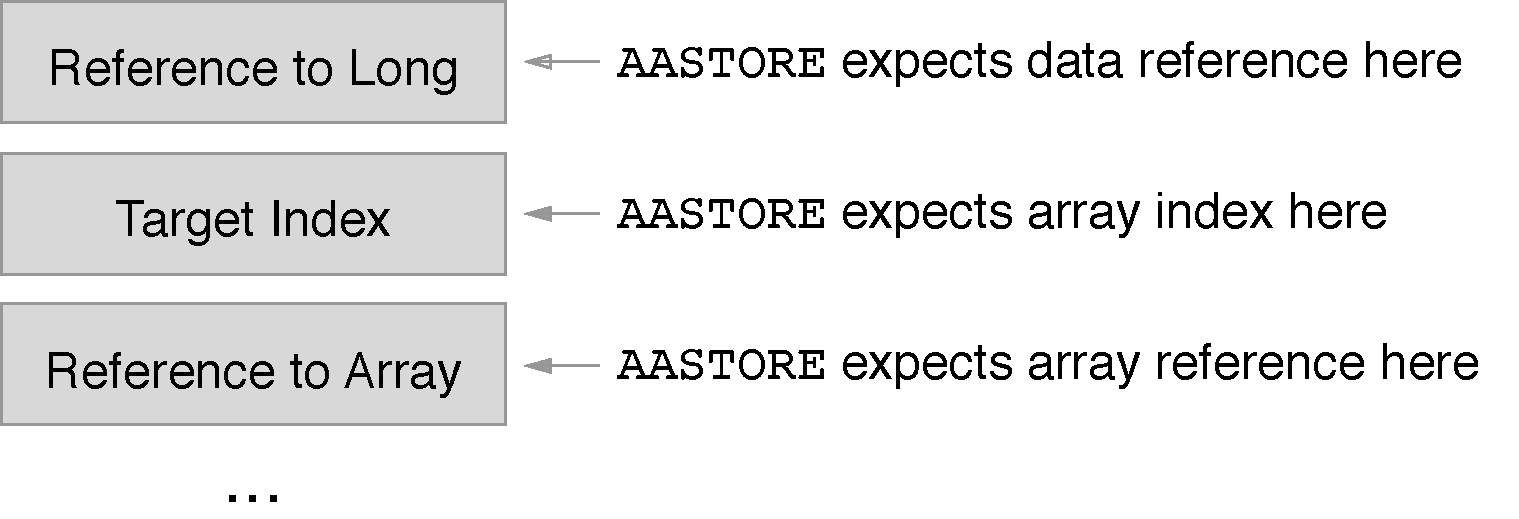
\includegraphics[scale=0.3]{figures/Correct_stack.pdf}
\caption{\small \sl Correct Operation of AASTORE \label{fig:correct_stack}}
\end{center} 
\end{figure}

This erroneous arrangement of the stack, where the primitive \lstinline{long} remains on the stack unboxed happens when the call to \lstinline{MethodVisitor.box(type)} is omitted. Because \lstinline{index} is a low number, intended to represent the target index in the target array, a \lstinline{SIGSEGV} from the operating system is virtually guaranteed when this low value is dereferenced. A Java stack trace will not result, only a JVM error.

\begin{figure}[!h]
\begin{center}
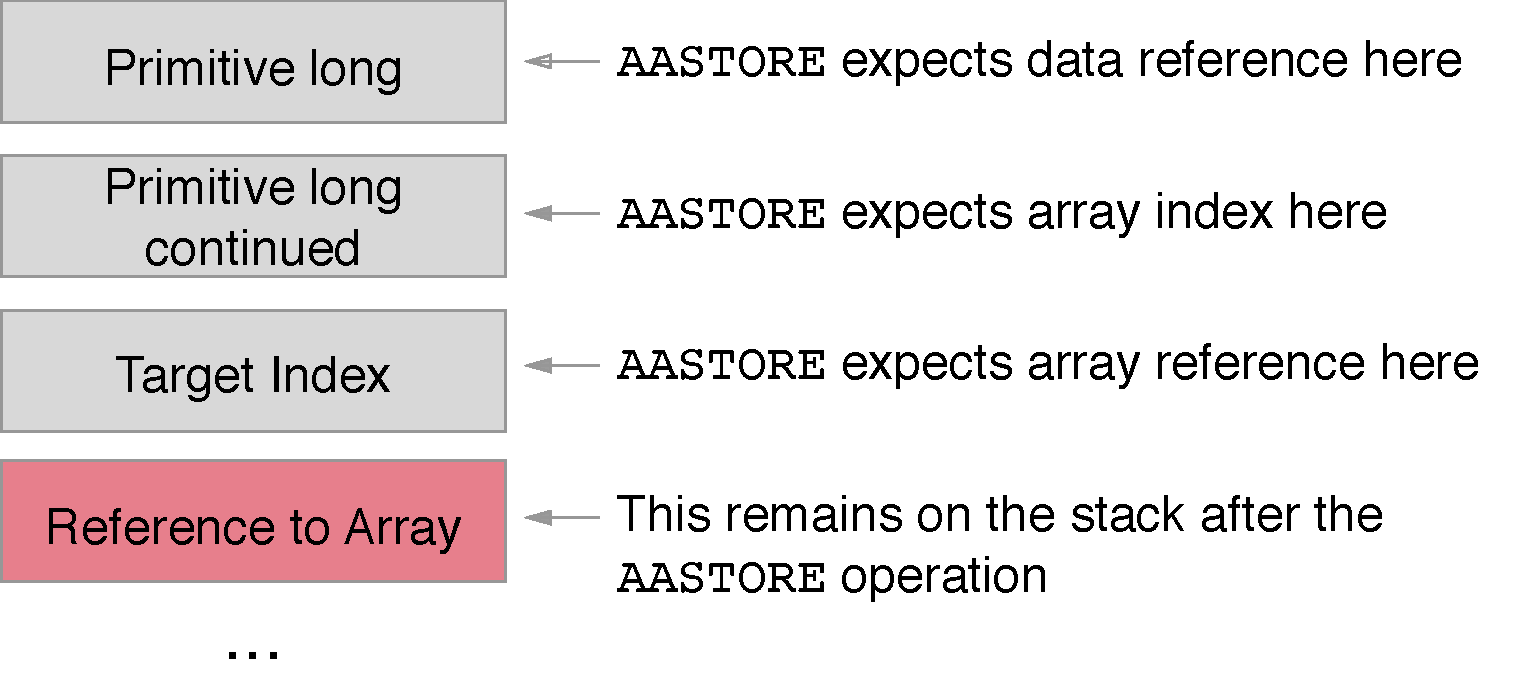
\includegraphics[scale=0.3]{figures/Incorrect_stack.pdf}
\caption{\small \sl Incorrect Operation of AASTORE \label{fig:incorrect_stack}}
\end{center} 
\end{figure}

\FloatBarrier

\subsubsection{Instrumented Method Invocations to Classes in Lower ClassLoaders \label{lower_classloaders}}

In Java a \textit{Class Loader} is responsible for finding the bytecode of a Java class by name and loading it into the JVM for use. Often this bytecode is read from disk, but it can be taken over the network, or a subclass of \lstinline{java.lang.ClassLoader}\noop{} can be provided that obtains the bytecode by any means the programmer cares to implement. A running Java program, however, has multiple class loaders, and one of them is always the \textit{bootstrap} (or \textit{primordial}) class loader, which is a part of the JVM rather than being implemented in the Java libraries. This bootstrap class loader is implemented in C in the JVM as it loads the first Java class into the JVM, along with all classes from the Java Runtime Jar \lstinline{rt.jar}, and in turn the Java implementation of \lstinline{java.lang.ClassLoader} which serves as the superclass for all subsequent class loaders. Thereafter it remains in the JVM to manage those classes loaded from \lstinline{rt.jar}\noop{}. Application classes provided in a Jar or on the classpath are loaded in child class loaders, which are implemented in Java as subclasses of \lstinline{java.lang.ClassLoader}.\noop{}

When one Java class references another, such as when it tries to create an instance of it, or call a method within it, the referenced class must be in the same or a higher class loader than that which loaded the referencing class. Classes cannot reference other classes in class loaders that are siblings or children of theirs.

Ordinarily this mechanism works just fine as classes are loaded in the highest class loader that has access to the definition of the class. Only in applications that change the behaviour of class loaders in an effort to have multiple versions of a class is this a problem. This can occur where a very common library, such as, for example, \textit{log4j}\footnote{\url{http://logging.apache.org/log4j/2.x/}} is loaded multiple times in an application but under different class loaders. Application Servers often encapsulate purely application code in a lower class loader than that used by the  classes comprising the Application Server itself, thus permitting multiple versions of common libraries, and eliminating namespace collisions between classes of the application server and code subsequently loaded into it.

A complication arises when instrumenting a class that has been loaded from \lstinline{rt.jar}, (Such as anything in the \lstinline{java.lang} package) as those classes are always loaded by the bootstrap class loader, and therefore cannot reference classes in any lower class loader. This is a problem if you wish to instrument such a class to call a method which you have provided with your agent or application code, as those are loaded by class loaders other than, and lower than, the bootstrap class loader, and so a \lstinline{NoClassDefFoundError}\noop{} will result at runtime.

In the context of the Mimic application, it is essential to instrument \lstinline{java.lang.Thread} to be notified when a new thread is constructed in the JVM. This is achieved by intercepting the method entry and exit on \lstinline{Thread.run()} in the same fashion as all other method interceptions. The inserted bytecode calls an accounting method, in this case \lstinline{Register.enter()} to notify the gathered parameters and, indirectly, the thread id (Because \lstinline{enter()} runs in the target thread, being invoked from \lstinline{Thread.run()}.)\noop{}

However this arrangement is only possible if the \lstinline{Register} class is available to the \lstinline{Thread} class and that is not routinely so because \lstinline{Thread} is in the bootstrap class loader as previously described. It is infeasible to move \lstinline{Thread} to a different class loader as classes cannot be unloaded, and it is required in the bootstrap class loader for the use of other classes also contained therein. Thus the obvious solution is to move the \lstinline{Register} class into the bootstrap class loader to cohabit with \lstinline{Thread} and all core classes from \lstinline{rt.jar}. This works well because the \lstinline{Register} class then becomes available to all classes because it is now in the topmost class loader.

To achieve this fix, the Jar file that contains the \lstinline{Register} class is loaded directly into the bootstrap class loader in the invocation of the JVM by using the command line option\linebreak[4] \lstinline{-Xbootclasspath/a:/path/to/my.jar}, where the named Jar contains the \lstinline{Register} class, either separated into its own Jar, or indeed by loading the Jar containing the entire Java agent and Mimic application, complete with \lstinline{Register} class into the bootstrap class loader. The second option introduces the Mimic application and related classes unnecessarily to the bootstrap class loader, but this is not a difficulty as they will simply be visible to every class loader in the JVM, and thus will not be re-loaded by any other class loader. Thus when bytecode in \lstinline{java.lang.Thread} is instrumented to include an \lstinline{INVOKESTATIC}, \lstinline{INVOKESPECIAL}, \lstinline{INVOKEVIRTUAL}, or \lstinline{INVOKEDYNAMIC} bytecode instruction that references the \lstinline{Register} class, it will succeed at runtime as the class \lstinline{Register} is now visible to the class \lstinline{Thread}.

\section{Performance Measurement}

Given an application that has been disconnected from its external dependencies using the techniques described in Section \ref{application_replay} it can now be run repeatedly without causing load on or affecting the state of other systems. In order to apply the techniques of application replay this project now proceeds to the practical demonstration of the Mimic application by devising a performance testing framework called \textit{Metre} that operates on a target application that has been instrumented with Mimic with a view to selecting the combination of Java Virtual Machine parameters with which the target runs most performantly.

The Metre application provided with the project artefacts implements a framework that repeatedly runs a Java application, each time using different JVM parameters drawn from a search pattern that is articulated in the Metre application configuration file.\footnote{The application configuration mechanism is implemented with XStream in the same manner as for the Mimic project artefact.} Each set of JVM parameters constructed from the search pattern is used to run the instrumented target application once and the combination of all runs is referred to as the \textit{experiment}. The end goal of the experiment is to:

\begin{itemize}
\item determine programmatically which collection of JVM parameters is best;\footnote{The term ``best'' in this context is the subject of further exploration in Subsection \ref{score_cards}}
\item provide the user with a graphical representation of critical metrics of the best performing program executions.
\end{itemize}

\subsection{Metrics Collection}
% the metrics fountain

Measuring the performance of the instrumented target application requires a selection of performance metrics spanning CPU, Memory, Garbage Collection, and also a measure of whether the invocation was successful.\footnote{Other metrics are available from the JMeter load test framework as discussed in Subsection \ref{application_of_load}.} A number of technologies were considered for collection of such performance metrics from the target application.

\subsubsection{Flight Recorder} 

The Oracle HotSpot JVM includes a feature called ‘Flight Recorder’. When activated, the JVM produces a textual record of metrics from the JVM for the duration of its execution.

Java Flight Recorder and Java Mission Control\footnote{\url{http://www.oracle.com/technetwork/java/javaseproducts/mission-control/java-mission-control-1998576.html}} are commercially available features for the collection of performance data from the JVM during execution that can be analysed afterward. The \textit{Oracle Java Mission Control} application can be used to configure the data collection performed by Flight Recorder, producing a settings file which can be passed on the command line to the JVM on invocation to direct the recording of metrics.

Unfortunately there are reasons why Flight Recorder is unsuitable for this project:

\begin{itemize}
\item Flight Recorder is a feature of \textit{Java SE Advanced} or \textit{Java SE Suite} which are not freely available, requiring instead a paid licence from Oracle;
\item Flight Recorder can be configured with a settings file specified as a command line argument to the JVM, and the settings file can be created in Oracle Java “Mission Control” as described, however the resulting settings file must be placed in a specific directory under the installed JVM in which the application under scrutiny is running, it cannot be provided programmatically by the Metre application;
\item The output of Flight Recorder is in the form of a log file. While this file could be parsed after the execution of the JVM, a scheme of real-time measurement that can be achieved transparently and programmatically would be preferable.
\end{itemize}

\subsubsection{Performance Summary JVM Parameters}

The Oracle HotSpot JVM has a number of options to print statistics related to its execution, for example \lstinline{-XX:+PrintGC}, \lstinline{-XX:+PrintGCApplicationConcurrentTime}, \lstinline{-XX:+PrintGCApplication-}\linebreak[4]\lstinline{StoppedTime}. Similarly named options print data about garbage collection.\linebreak[4]\lstinline{-XX:+PrintTenuringDistribution}\noop{} prints information about the occupancy of the various generations in the JVM memory model. For CPU utilisation, a Hprof\footnote{\url{http://docs.oracle.com/javase/7/docs/technotes/samples/hprof.html}} agent can be loaded in the JVM at invocation to monitor CPU statistics at defined intervals.

Unfortunately though, this approach is rather scattered, requiring a selection of JVM parameters, and the use of the hprof agent in a JVM that already has the Mimic agent loaded. This approach would leave the desired data in both files and the standard output of the execution, and significant parsing would be required to decipher the desired metrics.

\subsubsection{JConsole and JMX}

Ideally a selection of metrics would be available in a programmatically accessible form without the need to parse output files. A tool that provides this function is “JConsole” which is provided with the JVM. JConsole connects to a running JVM and displays a wide selection of metrics including CPU, heap and memory generations, threads, loaded classes and garbage collection, which are ideally suited to determine the performance of a JVM invocation.

The JConsole application gathers this information from the running JVM using MBeans that are read from the remote JVM by connecting to its MBean Server, which is built into the JVM. Only some simple configuration is required to allow connection to the MBean server of a JVM, and it can be performed programmatically on the command line at invocation. A large selection of metrics are thus accessible and JConsole then reads them at intervals.

This project uses the same scheme whereby it connects to the MBean server of the JVM under scrutiny and collects desired metrics at intervals. These metrics can then be used to programmatically calculate an overall performance score for the run of the application, and can also be used to produce graphs for the perusal of the user, showing the relative performance of different JVM parameter selections.

In order to achieve this collection a \lstinline{MetricsFountain}\noop{} class is provided that remains connected to the JMX server of the JVM under test. A \lstinline{SampleCollector}\noop{} class then collects \textit{slices} consisting of all metrics of interest at regular intervals as defined in the application configuration file. These metrics then constitute a time series, and form the basis of the graphs that Metre outputs as described in Subsection \ref{time_series}.

\subsection{Application of Load \label{application_of_load}}

Figure \ref{fig:scheme} shows the interaction of the major project artefacts, where application replay effected with Mimic takes the place of the upstream services and the load is applied to the application under test, in this case the Synonym Service REST web service. Whereas normally this load would be applied by downstream services, it is desirable to isolate the target application from those downstream service for the same reasons as its isolation from upstream services, namely that participation of the downstream services would cause them load and likely change their state.

The Scarpe tool discussed earlier is capable of applying load to its target application, which allows it to both \textit{drive} its target application and effect record and replay within the\linebreak[4]application\cite{joshi:2007}, however the Mimic tool is completely reactive: it will not call a method of the target application, it merely intervenes to record and replay method calls originating elsewhere. For this reason it is necessary to apply load to the target application while measuring its performance as otherwise it will not perform any work and performance measurement will be meaningless. In order to apply load to the target application the JMeter load test framework is used instead.

Use of the JMeter load test framework has three major advantages beyond decoupling the system from its downstream:

\begin{itemize}
\item the load is exactly repeatable each time;
\item performance measures become available in the JMeter log file;
\item the nature of the load and approximate runtime of each test run is known.
\end{itemize}

Conversely, one disadvantage is that the load applied might not correctly represent the load that the target application routinely experiences when installed in its normal place between real upstream and downstream systems, however this is a potential difficulty with any load testing endeavour and a representative load test script of short duration is assumed for the purposes of the experiment. 

\subsubsection{Log File Parsing}

The use of JMeter to apply load has the advantage that additional metrics are available for each invocation of the target application. The Metre application names the JMeter log file when it invokes the test script, and parses the test script immediately after the test run. These include the total run time, average, minimum, maximum test execution speed, and the number of tests that successfully passed. These metrics are written by JMeter as a single line in the log file, and can form an incremental result, which should be ignored, or a cumulative result. The last cumulative result in the log file is used. The test is considered successful only if all JMeter tests pass, and the resulting score is based on the run time of the test. Of course, more complicated scoring schemes and different tolerance to individual test failures are also possible.

\subsection{Target Execution}

The Metre application is also responsible for starting the target application for each set of JVM parameters. In each case, the target application takes some time to start up. Non-trivial target applications will usually need some time to be ready to process input, or in the case of the Synonym Service, to serve REST requests, and therefore a means is required to determine when an application is ready for load. Applying load too early is likely to cause test failures and will produce incorrect results on the initial tests which must wait.

While conceivably many techniques could be used depending on the behaviour of the target application, the technique implemented is to scan the output of the target application and seek a specific string. The \lstinline{TargetExecutor.start()}\noop{} method does not return until this string matches in the output.

The sequence of each test iteration is then:

\begin{itemize}
\item start the target application;
\item wait for the target's startup string;
\item start JMX metrics collection;
\item start the JMeter load test script and await its completion;
\item stop JMX metrics collection;
\item stop the target application.
\end{itemize}

\subsection{Specifying the JVM Parameter Search Space}

The Oracle Java HotSpot Virtual Machine accepts a very large number of command line parameters. Amongst the popularly known \textit{Non-standard Options} \lstinline{-Xmx} and \lstinline{-Xms} set the maximum size of the memory allocation pool and initial size of the heap respectively. However these two options are also available amongst the \textit{Advanced Runtime Options} as \linebreak[4] \lstinline{-XX:MaxHeapSize} and \lstinline{-XX:InitialHeapSize} \cite{java:2016}. Upon inspection, all parameters of interest are found to be included in the advanced runtime options, notwithstanding they may have legacy counterparts in the non-standard options. It is for this reason that the parameter selection focuses on the advanced runtime options: those beginning with \lstinline{-XX}.\noop{}

A complete list of available advanced runtime options for a given JVM can be obtained with the command \lstinline{java -XX:+PrintFlagsFinal -version}. These parameters accept values of these types: \textit{boolean}, \textit{integer}, \textit{string}, \textit{unsigned integer}, \textit{double}, \textit{unsigned 64 bit integer},\footnote{This can represent numbers that are too big for a \textit{long} type, by virtue of being unsigned, and thus cannot be represented by a Java primitive type, requiring instead a \textit{BigInteger}.} \textit{list of string}.

For the purposes of this project, only a subset of these parameters is implemented, specifically \textit{boolean}, \textit{integral}, \textit{string}. The large unsigned integer type and double type are excluded as they are not needed for the experimentation envisioned.

Each of the chosen parameter types is represented by a class that is capable of stepping through a range of values valid for that parameter:

\begin{description}[style=nextline]
\item[BoolParameter]  iterates through ``true'' and ``false'';
\item[IntegralStepParameter] iterates through a range of integers given a start and end of range, and a step value;
\item[StringListParameter] iterates through a list of strings.\footnote{These can also be string representations of integers if desired as they are used only to form the command line to invoke the target JVM.}
\end{description}

These are referred to as \textit{dynamic} parameters because their values can be iterated to form new collections of JVM parameters.

\begin{lstlisting}[language=xml,caption=Example of Specifying an \textit{IntegralStepParameter}]
<integralStepParameter>
    <!-- Percentage of the minimum free that, when used, triggers a CMS collection, 70 or 90 % -->
    <name>CMSTriggerRatio</name>
    <description>Percentage of Minimum Free Used to invoke CMS</description>
    <increment>20</increment>
    <maxValue>90</maxValue>
    <value>70</value>
</integralStepParameter>
\end{lstlisting}

\subsection{Special Examination of Garbage Collectior Parameters \label{special_garbage}}

In the course of designing the Metre application, and during initial experiments, an important discovery was made regarding parameters to the JVM that specify the Garbage Collectors to use. In a brief experiment, every possible combination of GC related JVM parameters was invoked, and the resulting selected Garbage Collectors were printed using a small class that queries the local JMX server. Specifically it was discovered that the actual number of \textit{combinations} of Garbage Collectors is quite small, numbering seven.

\begin{description}[style=nextline]
\item[Young Copy and Old ConcurrentMarkSweep] -XX:+UseConcMarkSweepGC -XX:-UseParNewGC
\item[Young Copy and Old MarkSweepCompact] -XX:+UseSerialGC
\item[Young G1 and Old G1] -XX:+UseG1GC
\item[Young ParNew and Old ConcurrentMarkSweep] -XX:+UseConcMarkSweepGC
\item[Young ParNew and Old MarkSweepCompact] -XX:+UseParNewGC
\item[Young PS Scavenge and Old PS MarkSweep] -XX:+UseParallelGC -XX:+UseParallelOldGC
\end{description}

In this list only one of the possible parameter selections is included for each Garbage Collector combination as there may be many, thus the most meaningful and intuitive selection is shown. This has important implications for the Metre configuration file and the search pattern it represents, as there is no purpose to exploring combinations of parameters that specify Garbage Collector selection other than those included in this list, though there are other parameters related to GC that do \textit{not} serve to specify the collector, and these may still form the basis of experiment.

\subsection{Static and Dynamic Parameters}

In order to accommodate the findings from Subsection \ref{special_garbage} a second type of parameter is introduced, referred to as the \textit{static} parameter. These are specified in the Metre application configuration and consist of a string of one or more JVM parameters, with associated values, which is incapable of iterating, always being included in the command line of the target JVM invocation in its literal entirety or not at all. The combinations of CG related parameters from Subsection \ref{special_garbage} are then perfectly accommodated and the distinct meanings of the specific parameter combinations is thus represented.

\subsection{Configuration Structure}

As a result of the findings of Subsection \ref{special_garbage} the structure of the configuration file for the Metre application comes to resemble that shown in Figure \ref{fig:search_pattern} where the static parameters are the seven parameter combinations that specify the Garbage Collector, and other dynamic parameters that iterate through strings, integers or booleans as appropriate. Some dynamic parameters exist at the highest level and iterate their values, these parameters are then combined with \textit{one} of the static parameters, which specifies the Garbage Collector to use, and then each Garbage Collector has within more dynamic parameters which iterate through their values.

\begin{figure}
\begin{center}
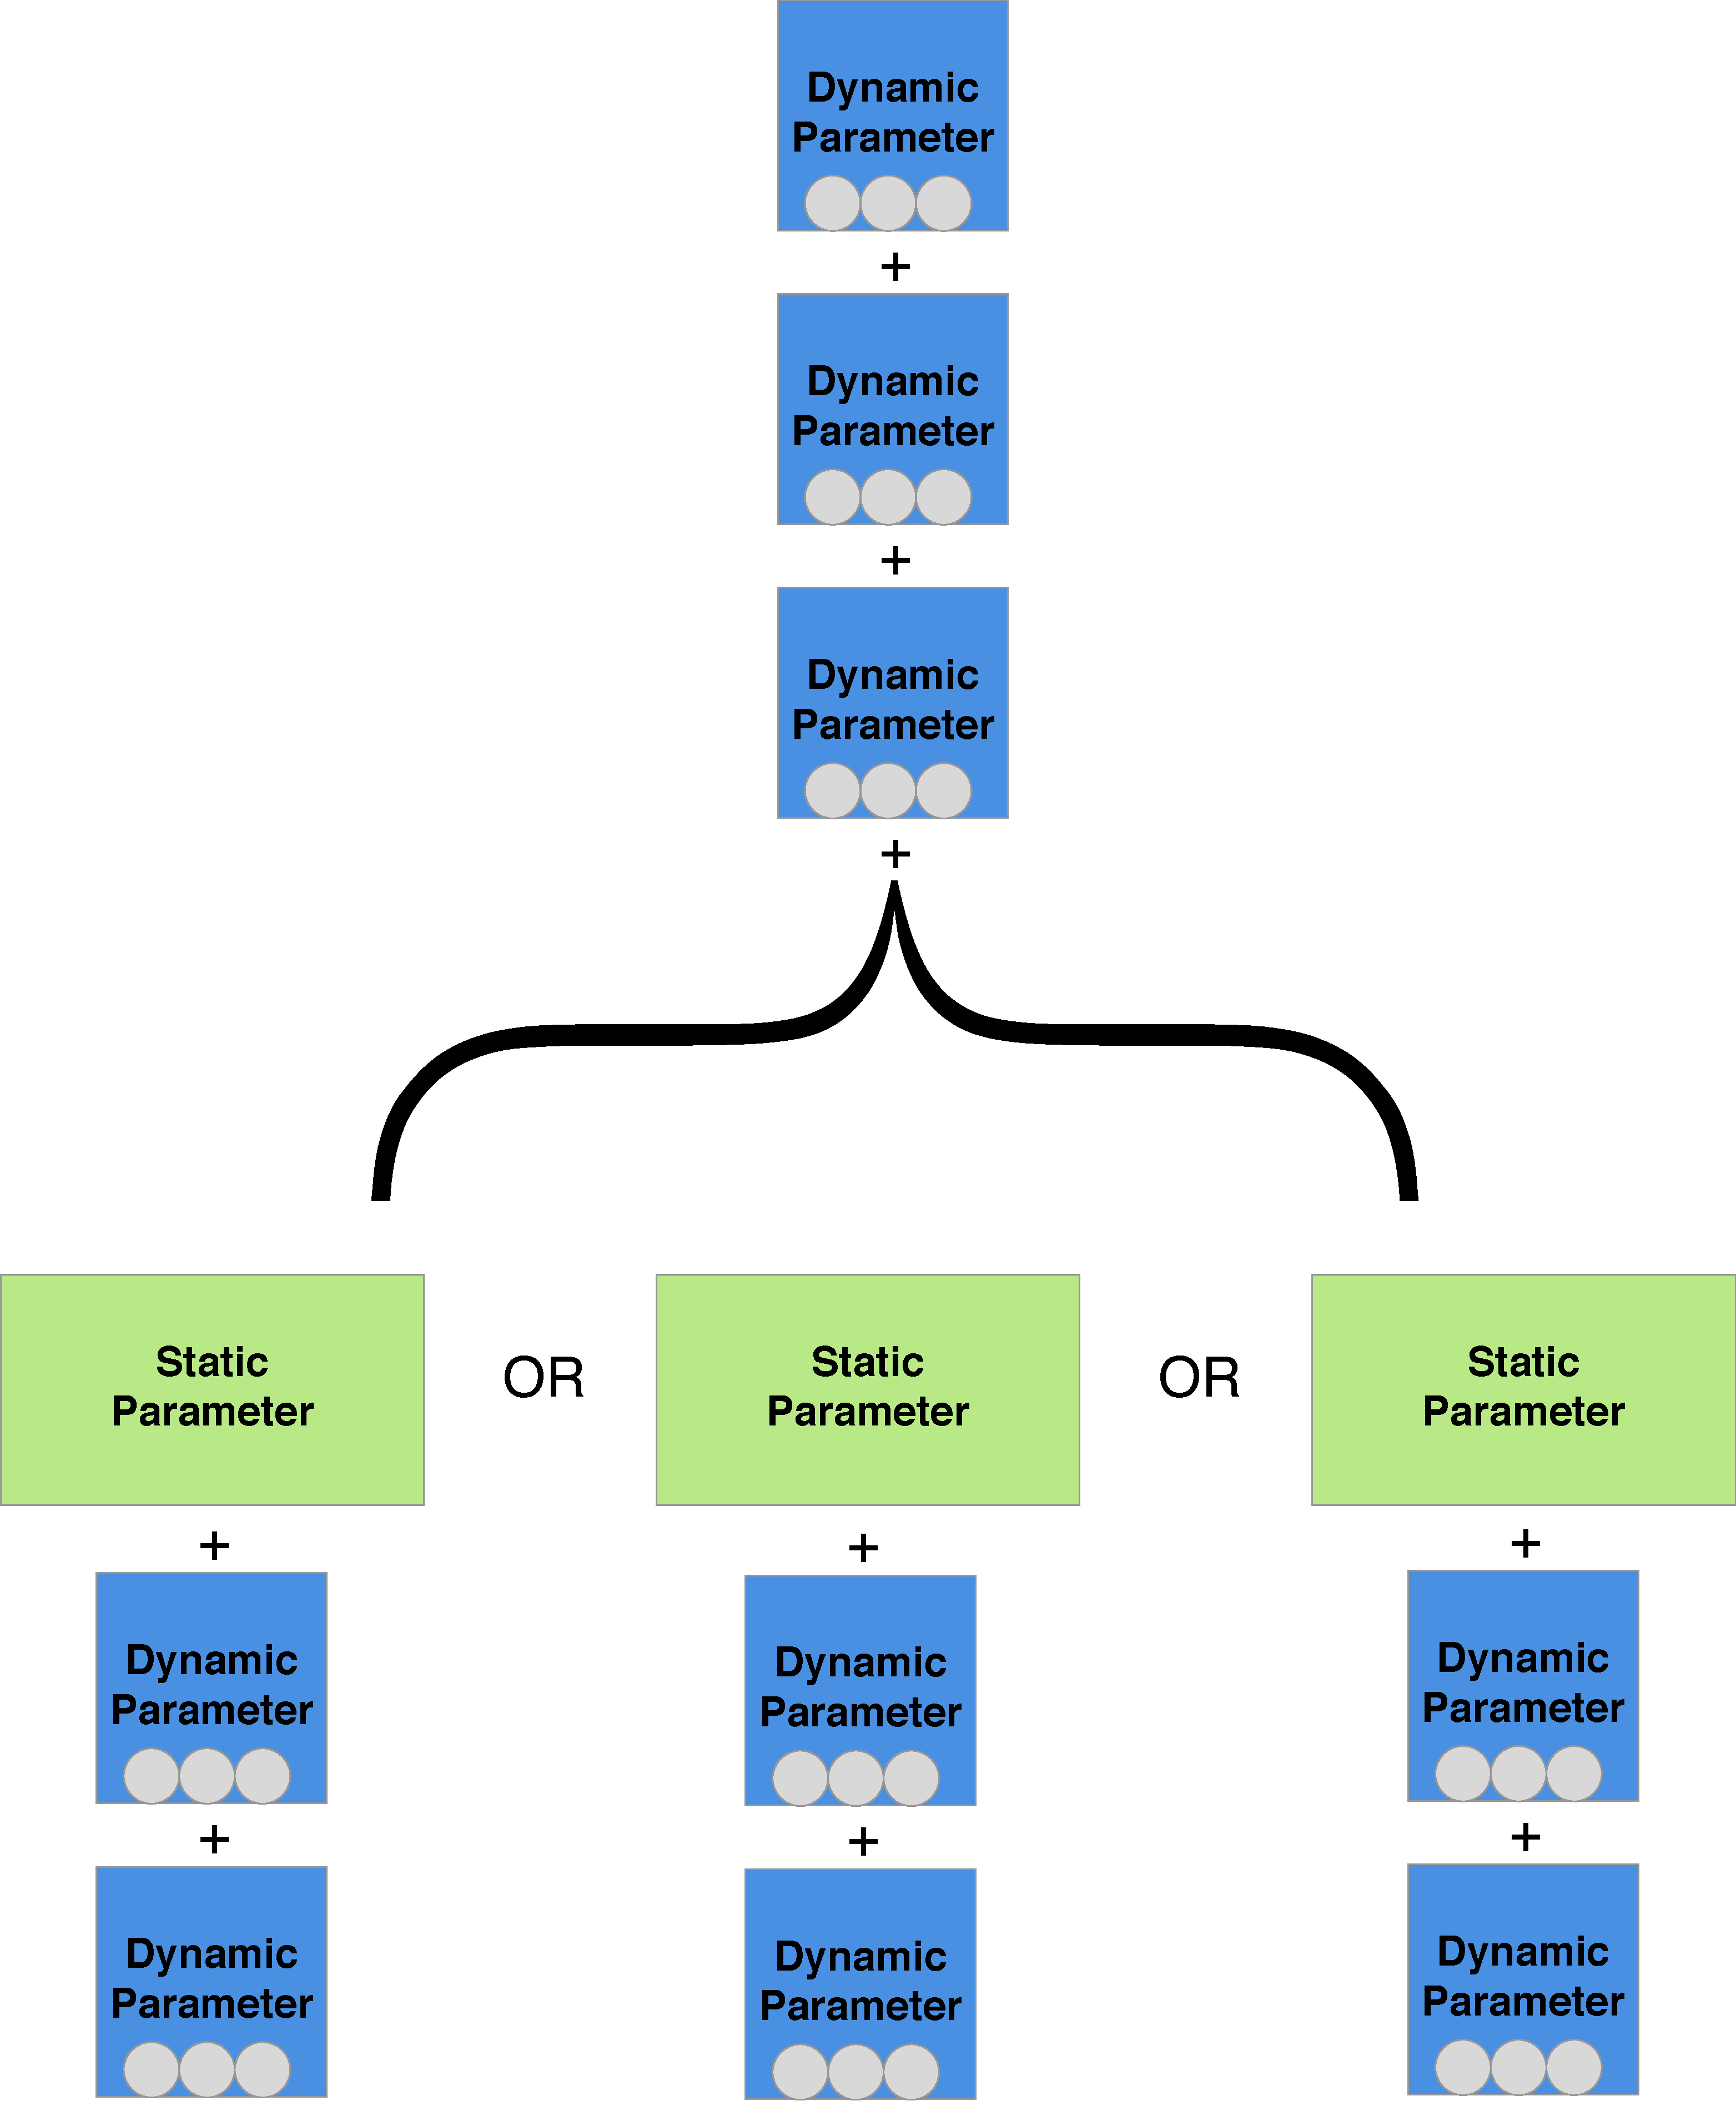
\includegraphics[scale=0.15]{figures/Search_Pattern.pdf}
\caption{\small \sl High Level Search Pattern for Metre \label{fig:search_pattern}}
\end{center} 
\end{figure}

The complete Metre configuration file used in subsequent experiments is included in Appendix A.

\subsection{Score Cards \label{score_cards}}

In order to record and represent the results of each JVM invocation a \lstinline{ScoreCard}\noop{} class is defined which stores the time series data and cumulative results taken from both the JMX metrics, and the JMeter log file. These are then stored in a \lstinline{ScoreTable}\noop{} which is implemented as a sorted set. The cards in the table are sorted in descending order of \textit{score}. The score measure is calculated from the data in the card at the time of creation, immediately after the JMeter test script completes. In these experiments the score has been calculated as the inverse of run time or $10,000/run time$ where the arbitrary multiplier provides for legibility.

More complex scores could be envisioned, however all time-related metrics, such as total time spent in GC are represented within run time. If performance characteristics relating to memory behaviour or GC pause times were required these could form the basis of the score but for the purpose of all experimentation here documented the inverse runtime score is used.

\subsection{Visualisation of Time Series Data \label{time_series}}

At the end of the experiment, the score cards are sorted and the cards with the top \textit{n} scores are selected, where \textit{n} can be specified in the configuration file. Each of these is then converted to a Gnuplot graph source file which can be plotted with the Gnuplot application, with the best performing being in \lstinline{scorecards/0001.gplot}.\noop{}

\subsection{Challenges to Measurement}
\subsubsection{The Attach API}

In order to connect to a remote JVM the class \lstinline{com.sun.tools.attach.VirtualMachine} from the Attach API is required along with supporting exceptions including \lstinline{AgentInitializationException}, \lstinline{AgentLoadException}, \lstinline{AttachNotSupportedException}. In order to use these classes it is necessary to include \lstinline{tools.jar}\noop{} in the classpath. This Jar file is provided with the installation of the Oracle HotSpot JVM version 1.8 but is not on the application classpath by default.

Ordinarily dependencies are introduced into the artefacts in the project by adding them to the pom.xml of the Maven build system. However \lstinline{tools.jar}\noop{} is a system dependency in that it is provided with the JVM, and the copy that is provided with the JVM is the correct one to use for applications executed with that JVM so it is not desirable to introduce tiirkheddlhvrjgeufhclljgvkirbvte\lstinline{tools.jar}\noop{} anywhere in the project or carry it around with the project. Instead the \lstinline{tools.jar}\noop{} must be referenced from its location in the JVM installation root both for the purposes of development and compilation with Maven and also at runtime when the compiled application executes.

To include a system dependency with Maven\footnote{\url{https://maven.apache.org}} is relatively simple, requiring this addition to the pom.xml:

\begin{lstlisting}[caption=Including a System Dependency with Maven, label={include_maven}]
<dependency>
    <groupId>jdk.tools</groupId>
    <artifactId>jdk.tools</artifactId>
    <version>jdk1.8.0</version>
    <scope>system</scope>
    <systemPath> ${java.home}/../lib/tools.jar </systemPath>
</dependency>
\end{lstlisting}

Listing \ref{include_maven} demonstrates referencing the system dependency relative to the Maven \lstinline{java.home}\noop{} location.

However, this will not make \lstinline{tools.jar}\noop{} available at runtime. In order to do so it must be added to the runtime classpath. The artefacts in this project all run from Jar files as they are packaged neatly by Maven. When they are executed using \lstinline{java -jar …}\noop{}on the command line, the classpath as defined by the Jar file cannot be extended by the addition of a command line option as it could be when executing a class directly.

For this reason the Metre artefact has one prerequisite activity which, while not ideal, is the neatest of the available options, specifically that the \lstinline{tools.jar}\noop{} file should be moved, copied or linked into the \lstinline{jre/lib/ext} directory, thereby installing it as an extension Jar for all invocations of the JRE that owns the \lstinline{jre/lib/ext} directory.\cite{extensions:2016}

Once this preparatory step is taken, invocation of the Metre artefact, as later described, but with the useful addition of the \lstinline{-verbose}\noop{} flag, will indicate that the relevant classes are loaded from \lstinline{tools.jar}\noop{} in its new location:

\begin{lstlisting}
[Loaded com.sun.tools.attach.AttachNotSupportedException from file:/Library/Java/JavaVirtualMachines/jdk1.8.0_65.jdk/Contents/Home/jre/lib/ext/tools.jar]
\end{lstlisting}

%% Experimental Design %%
\chapter{Experimental Design \label{experimental_design}}
\section{Synonym Service \label{synonym_service}}
In order to apply the technique of application replay to conduct a performance experiment, a target application is required. While multiple small single- and multi-threaded toy applications are explored in Chapter \ref{results_and_analysis}, the primary target of experimentation is a representative, if simplified, example web service built using Spring Boot which runs in a Tomcat\footnote{\url{http://tomcat.apache.org}} container, called \textit{Synonym Service} which has been constructed for the purposes of this project.

Synonym service is a HTTP REST service which accepts a block of text and attempts to find another block of text that has the same message digest as the original text as described by Daum and Lucks (2005) \cite{daum:2005}. The technique employed is to replace words in the original text with their synonyms drawn from an external upstream service. The Mimic application is then used to record interaction with that upstream service for a given JMeter script, such that the replay schedule can serve to satisfy re-runs of the JMeter script without upstream communication.

\begin{table}[]
\begin{center}
\begin{tabular}{p{0.15\linewidth}p{0.1\linewidth}p{0.3\linewidth}p{0.3\linewidth}}
URL & Request Method & Return & Purpose \\ \hline
/md5/{digest} & POST & Job number & Begin a new job using the MD5 message digest \\ \hline 
/bsd/{digest} & POST & Job number &  Begin a new job using the BSD Sum message digest \\ \hline
/{id}/progress & GET & An arbitrary incrementing progress number & Requests the stage of computation (progress) of the task with job number of \textit{id} \\ \hline
/{id} & GET & The result of the job run or the progress number in the Task-Progress HTTP header if not complete & Request the result of the job with job number \textit{id} \\ \hline
/{id} & DELETE & No return & Deletes the job from the system where the job number is \textit{id} \\ \hline
/status & GET & A textual list of all jobs in the system that have not been collected & Requests a list of all jobs, be they in progress or complete where the result has not yet been collected \\ \hline
\end{tabular}
\caption{REST Operations Supported by the Synonym Service}
\end{center}
\label{table:rest_operations}
\end{table}

\subsection*{Randomised Combination Iterator}

While not essential to the objective of the synonym service, in terms of either creating load, or in terms of finding message digest collisions, the order in which synonyms are substituted into the text is pseudorandom. However, if each substitution were chosen at random then there is the possibility to duplicate interim results and so a search pattern that exhausts the search space in a pseudorandom order but without revisiting any state is provided.

Every word in the input text that is not found in an included list of stopwords\footnote{Stopwords are uninteresting words like ``the'' or ``and''.} is expanded into its synonyms by calling the upstream service.

\begin{figure}
\begin{center}
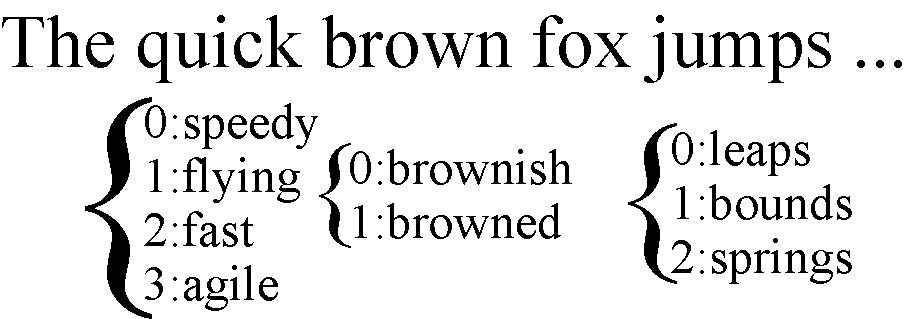
\includegraphics[scale=0.4]{figures/Word_Iterate.pdf}
\caption{\small \sl Synonym Expansion in Synonym Service \label{fig:word_iterate}}
\end{center} 
\end{figure}

The resulting structure, as shown in Figure \ref{fig:word_iterate} is a multidimensional array of inconsistent lengths composed of synonyms corresponding to words in the text which they can plausibly supplant without changing the meaning of the text.

While it might seem natural to iterate through all words in position 0 first, before proceeding to once increment position 1 and proceed thus much like a digital clock or car odometer, instead a layer of indirection is introduced such that the order of iterating through the words is randomised, much as if the individual dials of an odometer were shuffled such that the natural order (1000s, 100s, 10s, units) were randomised. Iterating through all combinations with this layer of indirection in place means that the search space is expanded without duplication, however because the indirection is itself randomised on each run, if a matching result is found it is highly likely to be different each time, especially for the BSD Sum digest which is easy to crack.\footnote{Solving the problem for the MD5 message digest on commodity hardware takes an infeasible number of years with this na\"{\i}ve approach, and while it is suitable for generating load, it is not used in this experiment as the JMeter test script would not terminate in reasonable time.}

\section{JMeter Load Test Script}
Because the Metre application does not provide a mechanism to apply load automatically, it uses instead a JMeter test script and a copy of the Apache JMeter software. The configuration file for Metre contains enough information to start JMeter with the desired load script. The location of the output log file is also specified, and Meter reads and interprets this log file after each execution of the script, taking from it the last non-incremental statistics line which represents the summary of all statistics during the JMeter execution.

A load test script for JMeter has been prepared that applies load to the Synonym Service REST client. The test script used in the experiments starts 25 BSD Sum tasks, polls the status operation until all jobs are complete and then reaps all jobs. This concludes one iteration of the test script.

\section{Description of the Test Environment}

In order to run the performance experiment, a workplace directory is created which contains the following key components:

\begin{description}
\item[Config.xml] \hfill \\  the configuration file for Metre, as in Appendix A;
\item[SynonymServiceIsolatorConfig.xml] \hfill \\  the configuration for Mimic to conduct application replay on the Synonym Service, as in Appendix B;
\item[apache-jmeter-2.13.tar] \hfill \\  Apache JMeter;\footnote{As obtained from \url{http://jmeter.apache.org/download_jmeter.cgi}}
\item[jmeter] \hfill \\  a directory containing the contents of \textit{apache-jmeter-2.13.tar};
\item[jmeter.jmx] \hfill \\  a JMeter test plan of short duration;
\item[metre-1.0.0-jar-with-dependencies.jar] \hfill \\  the compiled result of the Metre project artefact with no external Java dependencies;
\item[mimic-1.0.0-jar-with-dependencies.jar] \hfill \\  the compiled result of the Mimic project artefact with no external Java dependencies;
\item[synonym-service-1.0.0.jar] \hfill \\  the compiled result of the Synonym Service project artefact.
\end{description}

In the course of running the performance experiment, the following files and directories are created:

\begin{description}
\item[SynonymService\_cache.bin] \hfill \\ the output of the Mimic record phase that informs subsequent replay;
\item[application.log] \hfill \\  the log file of the Metre application;
\item[jmeter.log] \hfill \\  the log file of \textit{the previous} JMeter invocation performed by Metre;
\item[scorecards] \hfill \\  a directory containing the output of the top \textit{n} score cards in Gnuplot format.
\end{description}

\begin{table}
\begin{center}
\begin{tabular}{ll}
\hline
OS & OS X ``El Capitan'' with Darwin Kernel Version 15.4.0 \\ \hline
Memory & 8GB \\ \hline
CPU & 1.7 GHz Intel Core i7 \\ \hline
JVM & Java HotSpot(TM) 64-Bit Server VM version ``1.8.0\_9'' \\ \hline
JDK & Oracle Java JDK1.8.0\_65 \\ \hline
\end{tabular}
\caption{Key Features of the Test Platform}
\end{center}
\label{table:key_features_test}
\end{table}

\FloatBarrier

\section*{The Record Phase}

The record phase is conducted with a command of this form:

\begin{lstlisting}
java \
    -Xbootclasspath/p:mimic-1.0.0-jar-with-dependencies.jar \
    -javaagent:mimic-1.0.0-jar-with-dependencies.jar\
        =replay,SynonymServiceIsolatorConfig.xml \
    -jar synonym-service/target/synonym-service-1.0.0.jar
\end{lstlisting}

The configuration, as listed in Appendix B, specifies the functional application replay mechanism and so the output deposited in the file \lstinline{SynonymService_cache.bin}\noop{} represents all possible parameters to the instrumented method \lstinline{getSynonyms}\noop{} mapped to the recorded return from the upstream service.\footnote{If the \textit{reconciled} mechanism were specified, a number of per-thread scheduling and a summary files would be produced as in other examples.} The three parameters to the record command have the following meanings:

\begin{description}
\item[-Xbootclasspath] \hfill \\ places Mimic on the boot class loader as described in Subsection \ref{lower_classloaders};
\item[-javaagent] \hfill \\ specifies the Mimic Jar file to load as an agent, with parameters specifying the mode (replay) and the configuration file name;
\item[-jar] \hfill \\ the target application to run and record.
\end{description}

In order to replay, the same command is used, with ``replay'' in place of ``record'' and then the load test script can be run against the Synonym Service instrumented for replay, and no connection to the upstream service results.

\section*{The Performance Experiment \label{performance_experiment}}

The Metre application is invoked by executing the \lstinline{metre-1.0.0-jar-with-dependencies.jar}\noop{} executable Jar file:

\begin{lstlisting}
java -jar ./metre-1.0.0-jar-with-dependencies.jar
\end{lstlisting}

The configuration is then read from \lstinline{Config.xml}. The configuration file used in this experiment is listed in Appendix A. The provided configuration is designed to trial each of the seven valid combinations of JVM parameters with a combination of dynamic parameters that iterate through values in a specified range. Some of the dynamic parameters are dependant on the GC selection, being within the \textit{statics} tag, and some have global applicability, being at the top level of the configuration structure within the \textit{dynamics} tag.

The provided configuration, when expanded, results in 1088 combinations of JVM parameters, though abstemious selection of JVM parameters and ranges to explore is required to make the number of combinations this small. The provided JMeter script runs in approximately two minutes, and so a complete performance run takes approximately 36 hours. The unfortunate length of this experiment is suggestive of future work.

Upon completion of the performance experiment, the top three invocations are taken and plotted. A sample Gnuplot output file is listed in Appendix C and the Gnuplot graphical output is shown in Chapter \ref{results_and_analysis}.

%% Results and Analysis %%
\chapter{Results and Analysis \label{results_and_analysis}}

\section*{Application Replay Experiments}

\subsection*{Console Conversation \label{console_conversation}}

A small console-based application is used to test the basic functionality of instrumentation in a single-threaded application. The application is presented in Appendix D, though its function is only to ask some questions of the user and respond formulaically with preposterous answers. The application can be recorded as the user answers the questions, and upon replay the answers are reiterated on the console. User interaction is correctly recorded and replayed by instrumenting the method \lstinline{java.io.Console.readLine()} which returns a \lstinline{String}. Correct responses on replay are an indication of correct record and replay, and the delay that the user caused while typing a response is simulated as it happens inside the recorded method. The end result is an amusing effect of an invisible user.

\begin{lstlisting}[language=xml, caption=Mimic Configuration to Record and Replay a Console Conversation, label={converse_mimic_config}]
<mimicConfig>
  <basename>Converse</basename>
  <mechanism>reconciled</mechanism>
  <classMatch>
    <classPattern>java.io.Console</classPattern>
    <methodMatch>
      <methodPattern>readLine</methodPattern>
      <regex>false</regex>
      <signatureEquals>()Ljava/lang/String;</signatureEquals>
    </methodMatch>
    <regex>false</regex>
  </classMatch>
 </mimicConfig>
\end{lstlisting}

The Mimic configuration used in this experiment is shown in Listing \ref{converse_mimic_config}. An interesting artefact is observed when the line \lstinline{<signatureEquals>()Ljava/lang/String;</signatureEquals>} is altered to \lstinline{<signatureMatches>.*</signatureMatches>} thereby matching both methods\linebreak[4]\lstinline{readLine(String, Object)} and \lstinline{readLine()}. It appears that the method with no arguments internally calls the method with two arguments, and if both are instrumented then the recorded schedule includes information for both invocations. However methods on replay do not have any body beyond that required to return the recorded result and simulate the original delay, and therefore there is unused information in the recorded schedule that causes incorrect replay in the case of instrumenting methods that are called by other instrumented methods. While not an intractable problem, a means to discard recordings from the nested calls to instrumented methods is indicated for future work.

\subsection*{Simple Threaded Application \label{simple_threading}}

A simple multi-threaded application is presented in Appendix D as an example of simple threading. The reason that it is considered \textit{simple} is that \lstinline{Thread.start()}\noop{} is called for each thread on a different line. Therefore each invocation of \lstinline{Thread.start()}\noop{} has a different stack trace. The application is instrumented with the configuration in Listing \ref{natural_mimic_config}.

\begin{lstlisting}[language=xml, caption=Mimic Configuration to Record and Replay a Simple Threaded Application, label={natural_mimic_config}]
<mimicConfig>
  <basename>Threading</basename>
  <mechanism>reconciled</mechanism>
  <classMatch>
    <classPattern>org.overworld.mimic.sample.naturalthreading.MyThread</classPattern>
    <methodMatch>
      <methodPattern>getMyName</methodPattern>
      <regex>false</regex>
      <signatureMatches>.*</signatureMatches>
    </methodMatch>
    <regex>false</regex>
  </classMatch>
 </mimicConfig>
\end{lstlisting}

Upon record the instrumented method \lstinline{getMyName()}\noop{} returns the name of the thread, and also internally prints its name:

\begin{lstlisting}
Getting name: two
Getting name: three
Getting name: one
Getting name: four
Getting name: five
Getting name: six
one
three
five
six
two
four
\end{lstlisting}

On replay the \lstinline{getMyName()}\noop{} method no longer prints its generated name because it no longer has a body, though the return value is replayed:

\begin{lstlisting}
Replay Instrumenting org/overworld/mimic/sample/naturalthreading/MyThread getMyName ()Ljava/lang/String;
six
five
four
two
three
one
\end{lstlisting}

It is observed that the threads executed in a different order on replay, because it is not the intention of Mimic to force thread scheduling to repeat its ordering.

\subsection*{Complex Threaded Application \label{complex_threading}}

The simple threading example just presented has threads that start on different lines of the containing Java file. Appendix D presents the code of an example class that creates threads using a loop such that six threads are all constructed using a \lstinline{Thread.start()}\noop{} invocation that is located on just one line. This is a step closer to real-world applications, and is termed \textit{complex threading} for the purposes of this discussion. The configuration given in Listing \ref{natural_mimic_config} is unchanged except in that the name of the class under test has changed, but the mechanism of instrumentation and the name of the instrumented method are the same.

In this case the order of creation of the threads is used to generate the persistant thread identifiers so that threads have distinct record schedules despite being created on the same source line of the Java file. The output observed is not materially different to that presented for simple threading.

\section*{Performance Experiment on the Synonym Service}
In order to instrument the Synonym Service for application replay, the \textit{functional mechanism} described in Subsection \ref{mechanism} is applied to the method \lstinline{SeekTask.getSynonyms(String)} \noop{} resulting in the configuration listed in Appendix B. The Metre application is then invoked as described in Section \ref{performance_experiment}.

\begin{figure}[!h]
\begin{center}
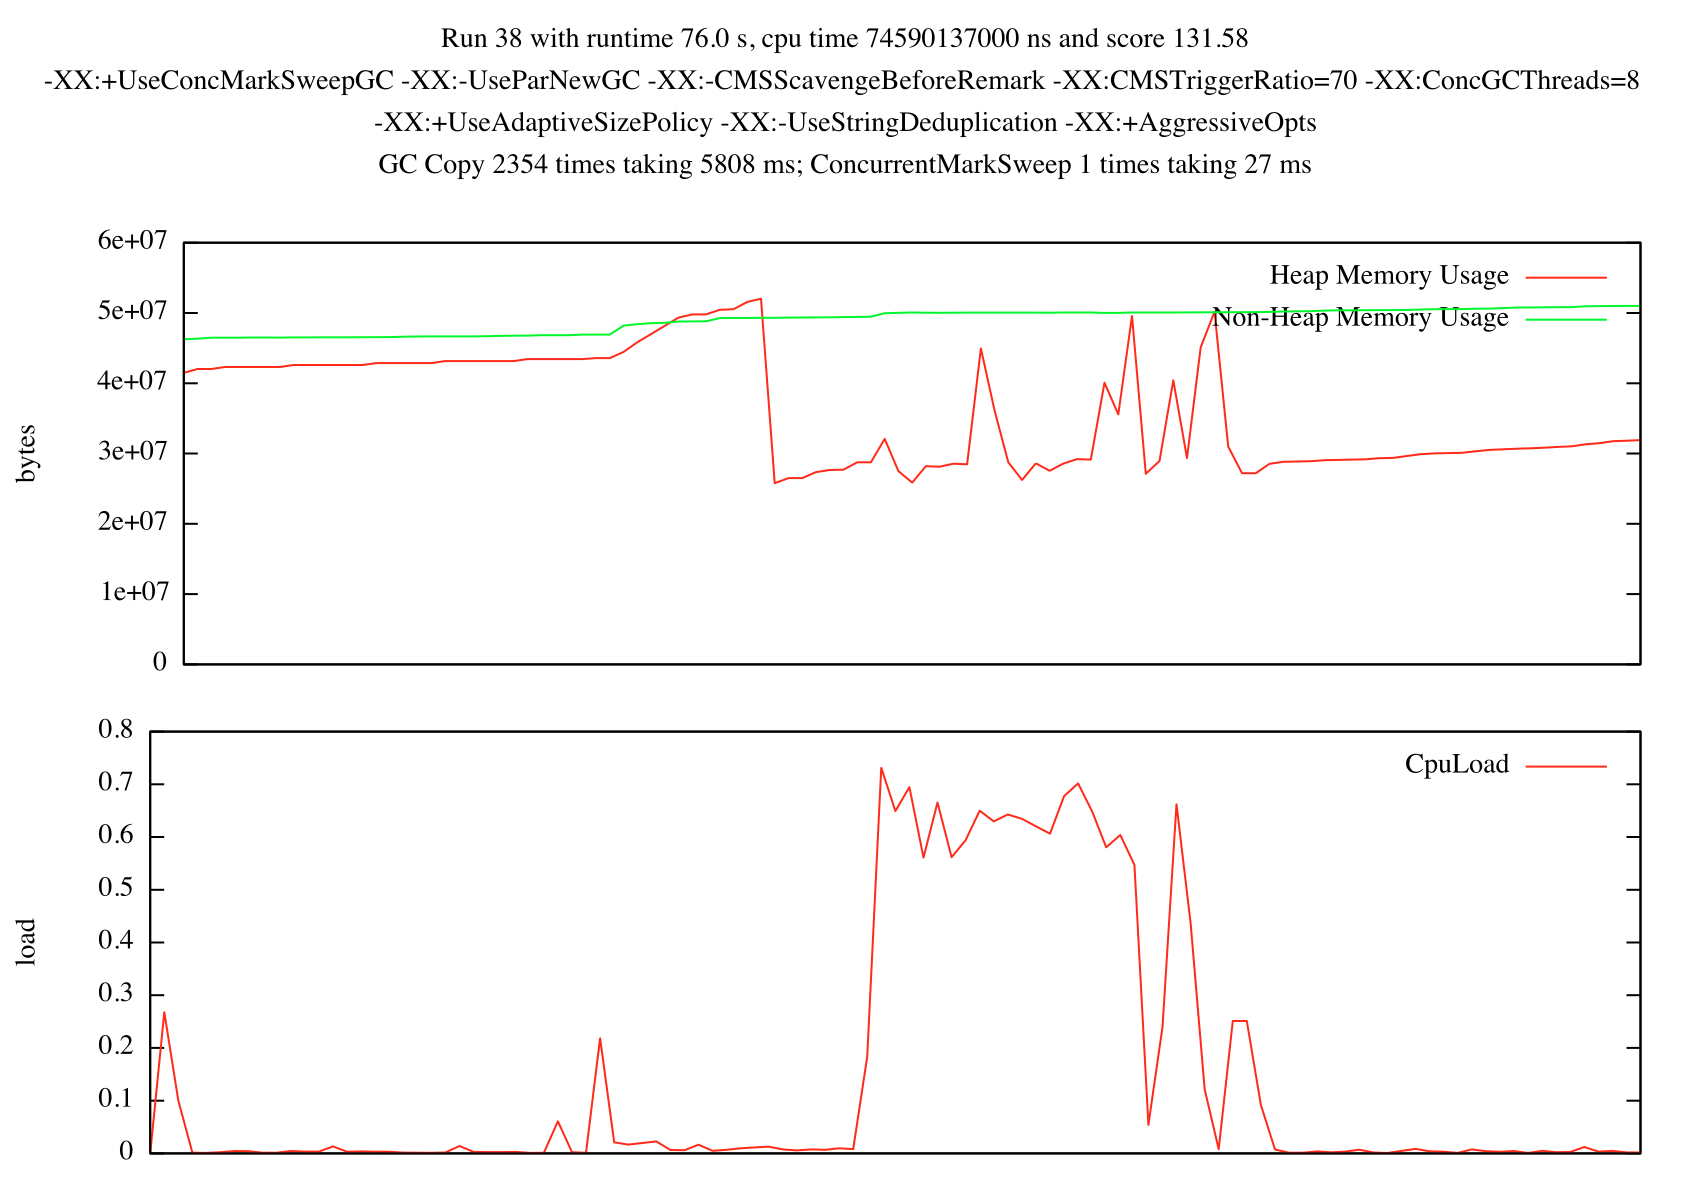
\includegraphics[scale=0.5]{figures/gplot_1.png}
\caption{\small \sl Output of the Most Performant Invocation of Synonym Service \label{fig0001}}
\end{center} 
\end{figure}

Upon completion of the experiment the invocation of the instrumented Synonym Service which took the shortest time is represented in the output file \lstinline{scorecards/0001.gplot} and shown in Figure \ref{fig0001}. The outputs of the second and third most performant invocation are included in Appendix E.

\begin{table}
\begin{center}
\begin{tabular}{lll}
Runtime & Young GC (Time) & Old GC (Time) \\ \hline
76.0s & Copy (5880ms) & ConcurrentMarkSweep (27ms) \\ \hline
78.0s & ParNew (7426ms) & ConcurrentMarkSweep (15ms) \\ \hline
79.5s & Copy (7014ms) & MarkSweepCompact (39ms) \\ \hline
\end{tabular}
\caption{Summary of GC Times of the Performance Experiment}
\label{table:summary_gc_times}
\end{center}
\end{table}

As noted in Subsection \ref{score_cards}, the score assigned to the invocation of the application is based on its run time. However if we examine the key GC metrics from the three most performant invocations, as shown in Table \ref{table:summary_gc_times}, we see that they have different Garbage Collector combinations for the young and old generations. Therefore, the runtime is not directly dependant on the selection of Garbage Collector.

%% Conclusion %%
\chapter{Conclusions \label{conclusions}}

It has been demonstrated that parts of an application can be disconnected from execution and that recorded values from an earlier execution of the application can be substuted using the techniques of application replay described in this report. Examples of application replay have been shown to be effective in stubbing out unwanted interactions in an application at a method level, and two mechanisms for correlating information between record and replay have been explored, specifically a \textit{functional} mechanism that assumes the method behaves as a function, always producing the same return value for a given set of parameters, and a \textit{reconciled} method that replays return values in the same order as they were recorded, while accounting for multi-threading, even where thread identifiers differ across multiple runs of the application. A substantive application with a Web Services architecture has been examined, and it has been subjected to application replay inside its Tomcat container. 

A performance measurement framework was then constructed which invokes an application repeatedly with different Java Virtual Machine parameters each time. The instrumented web service application, now disconnected from its upstream dependency, was placed inside the performance measurement framework and subjected to repeated execution without a connection to its upstream service which would normally provide required input, but instead having this input provided by the application replay mechanism.

During execution the application under test is monitored programmatically by the performance measurement framework using the Java Management Extensions server built into the Oracle HotSpot Java Virtual Machine so that each execution can be assigned a score to indicate the performance of its execution with the parameters selected for each iteration. The application is subjected to an identical load generated by the JMeter performance testing tool on each invocation, and the results of the load test also inform the score assigned to each invocation.

As the performance experiment was successful it is concluded that the technique of Application Replay has merit and is capable of disconnecting a non-trivial application from the dependencies which normally provide its input.

The performance measurement framework provided does have limitations though. It takes a brute-force approach to exploring the parameters to the Java Virtual Machine, and as such it takes a very long time to run even a modest test repeatedly to explore the effects of each combination of even a small number of JVM parameters. In the course of the experiment, seven Garbage Collector combinations and a total of not more than six JVM parameters for each were explored, this results in 1088 combinations to explore and, with a test script that executes to completion in two minutes, results in a 36 hour performance experiment.

Another limitation of the performance experiment is that each combination of parameters is the subject of only one invocation. If a variability is assumed, stemming from the underlying machine, operating system load, resource contention with other processes or other factors not controlled, then it would be preferable to perform each invocation multiple times and choose a modal result. However, as described, even a single invocation of each combination of JVM parameters results in a performance experiment of unwieldy duration. 

Ideally it would be possible to seek the most performant combination of JVM parameters without the need to visit every combination within a defined search pattern. It may then be possible to reduce the duration of the test. If a dramatic reduction were achieved then it may become feasible to perform repeated invocations to eliminate outliers. Alternatively (or additionally) it may be possible to conduct the performance experiment in a manner distributed over a large number of individual compute instances, especially if applied in a cloud environment. In this case there is the added complexity that the underlying cloud virtualisation technology may make the variability of results greater. These topics may provide areas of future work.

Turning back to application replay, while the technique shows both promise and practical applicability, it is fair to say that no \textit{one} mechanism has been perfected to successfully replay the correct input at the correct time that satisfies \textit{all} scenarios. Instead the \textit{reconciled} mechanism was explored which successfully replays invocations of a method in strict order within its thread of execution. The complexity of differing thread identifiers across invocations was addressed for simple example applications but a \textit{functional} mechanism was found more satisfactory when a more complex application more closely resembling a real-world system was explored. In order to improve the coordination of replay, more experimentation is required to reliably handle differing thread identifiers across invocations where the multi-threading in use reaches the complexity of a ThreadPoolExecutor and this may also serve as the topic of future work.

%% References %%
\newpage
\bibliographystyle{ieeetr}
\bibliography{report}

\chapter*{Appendix A: Metre Configuration File}
\addcontentsline{toc}{chapter}{Appendix A: Metre Configuration File}
\lstinputlisting[nolol=true]{includes/Metre_Config.xml}

\chapter*{Appendix B: Mimic Configuration File for Synonym Service}
\addcontentsline{toc}{chapter}{Appendix B: Mimic Configuration File for Synonym Service}
\begin{lstlisting}
<mimicConfig>
  <basename>SynonymService</basename>
  <mechanism>functional</mechanism>
  <classMatch>
    <classPattern>org.overworld.example.webservice.engine.SeekTask</classPattern>
    <methodMatch>
      <methodPattern>getSynonyms</methodPattern>
      <regex>false</regex>
      <signatureMatches>.*</signatureMatches>
    </methodMatch>
    <regex>false</regex>
  </classMatch>
 </mimicConfig>
\end{lstlisting}

\chapter*{Appendix C: Example Gnuplot Output File}
\addcontentsline{toc}{chapter}{Appendix C: Example Gnuplot Output File}
\lstinputlisting[nolol=true]{includes/0001.gplot}

\chapter*{Appendix D: Application Replay Experiments}
\addcontentsline{toc}{chapter}{Appendix D: Application Replay Experiments}
\section*{Instrumenting a Console Conversation}
\lstinputlisting[nolol=true]{includes/Converse.java}
This class is instrumented using the configuration presented in Chapter \ref{console_conversation}.
\newpage

\section*{Instrumenting Simple Threading}
\lstinputlisting[nolol=true]{includes/NaturalThreading.java}
This class is instrumented using the configuration presented in Chapter \ref{simple_threading}.
\newpage

\section*{Instrumenting Complex Threading}
\lstinputlisting[nolol=true]{includes/ComplexThreading.java}
This class is instrumented in Chapter \ref{complex_threading}.
\newpage

\chapter*{Appendix E: Additional Graphs of the Performance Experiment}
\addcontentsline{toc}{chapter}{Appendix E: Additional Graphs of the Performance Experiment}

\begin{figure}[!h]
\begin{center}
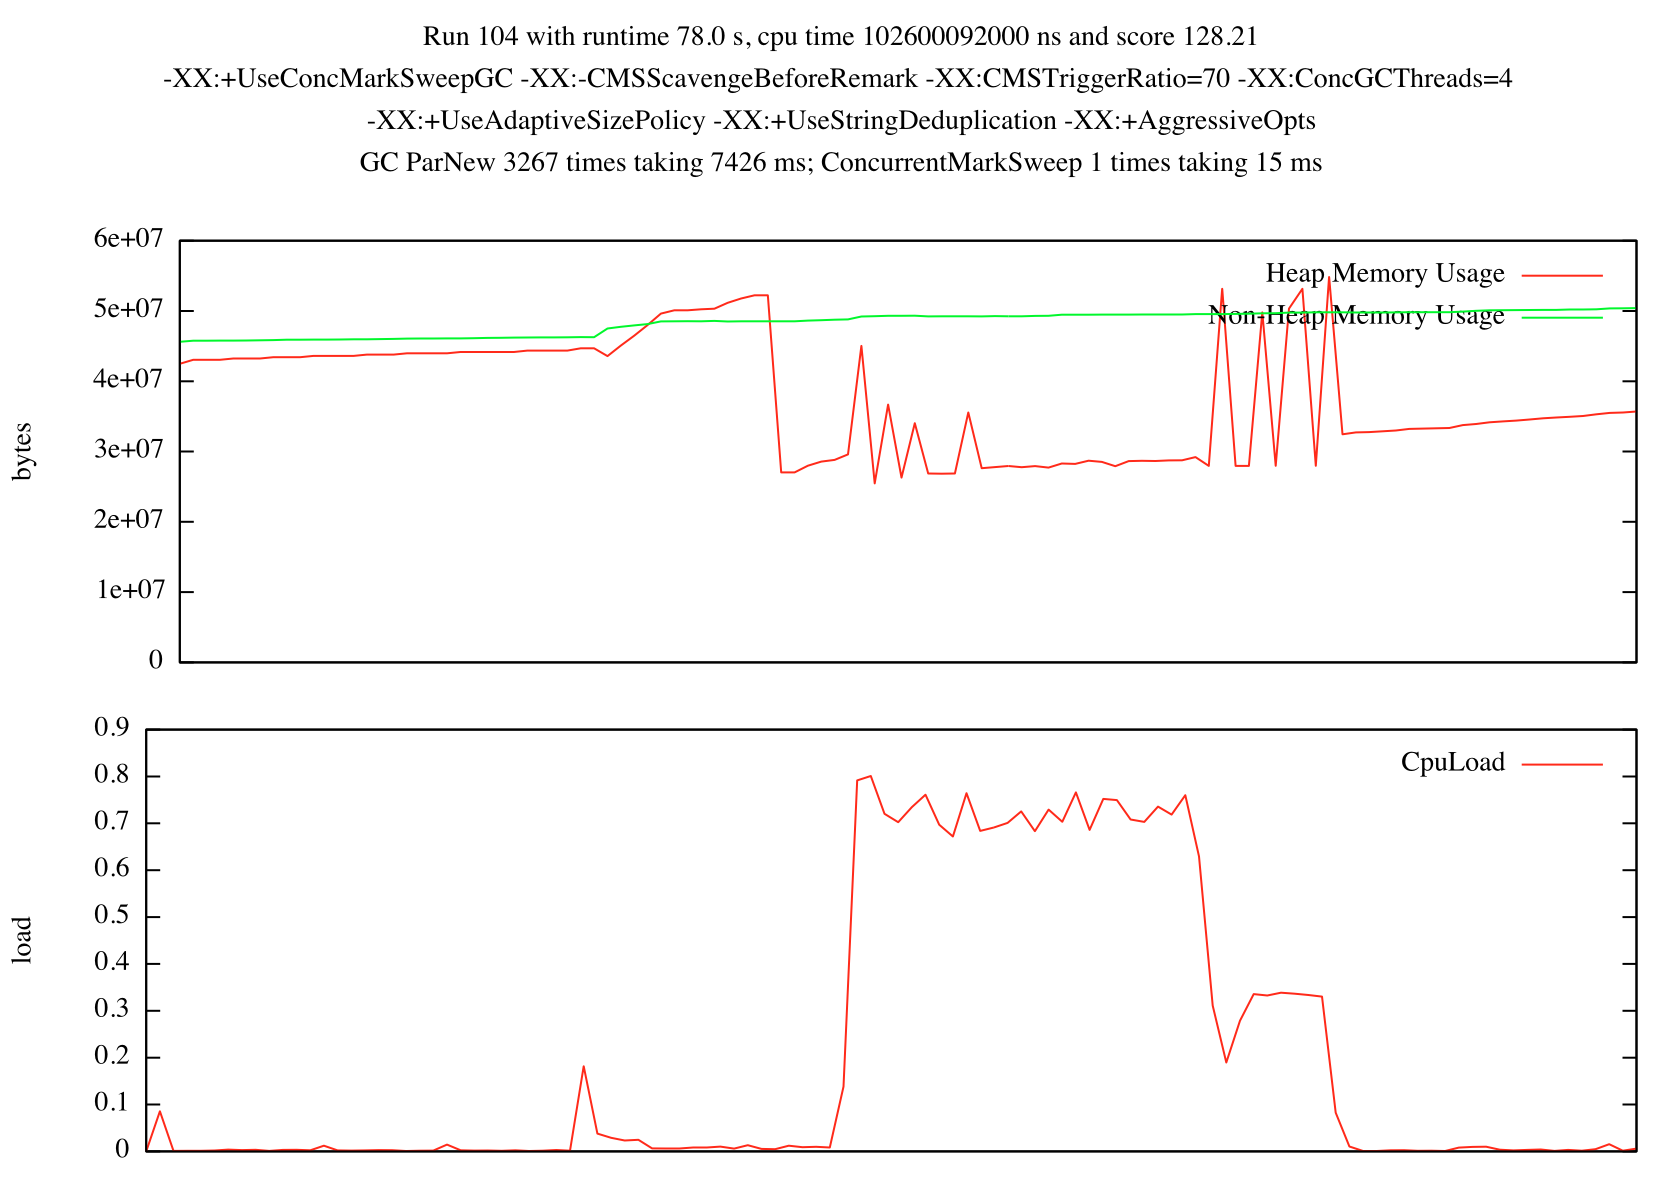
\includegraphics[scale=0.4]{figures/gplot_2.png}
\caption*{\small \sl Output of the Second Most Performant Invocation of Synonym Service}
\end{center} 
\end{figure}

\begin{figure}[!h]
\begin{center}
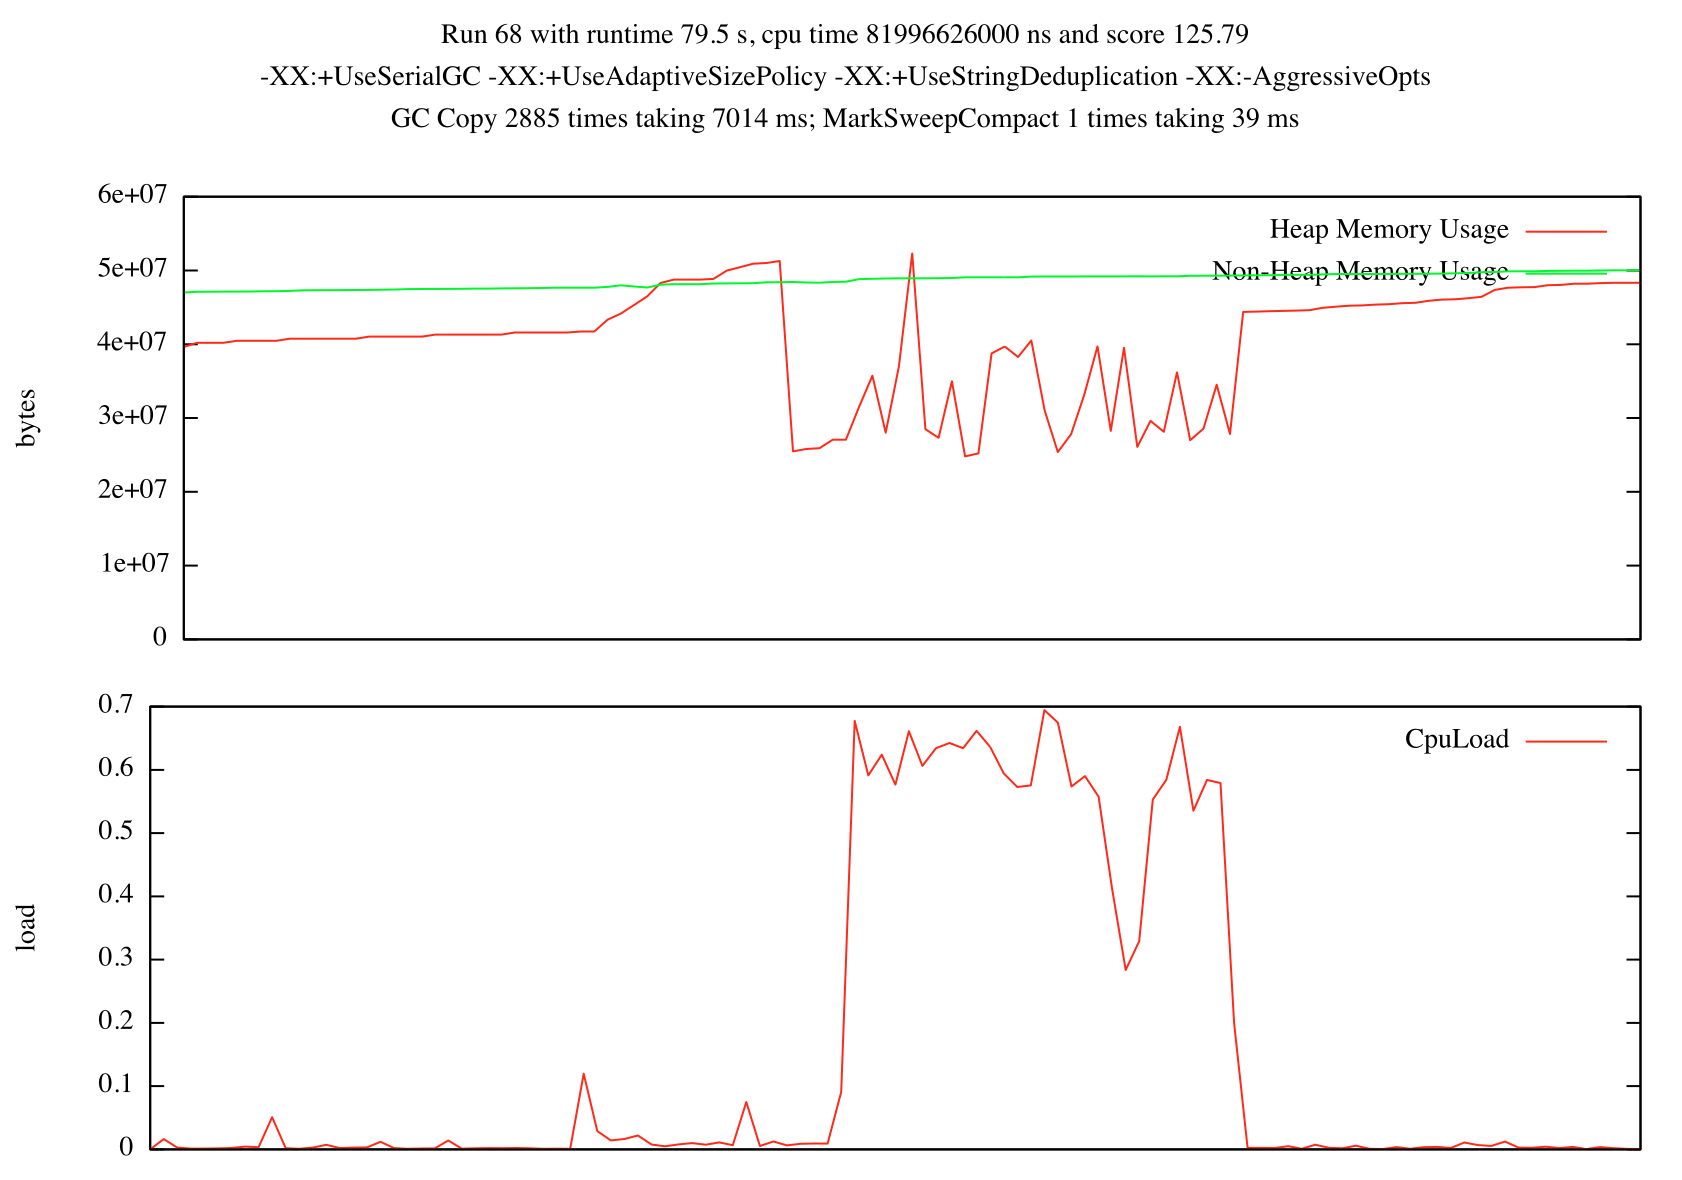
\includegraphics[scale=0.4]{figures/gplot_3.png}
\caption*{\small \sl Output of the Third Most Performant Invocation of Synonym Service}
\end{center} 
\end{figure}
\end{document}
\newpage